\documentclass[usenatbib]{rasti}

\usepackage{graphicx}
\usepackage{amsmath}
\usepackage{amssymb}
\usepackage{url}

% Draft version information
\newcommand{\draftversion}{V1.12}
\newcommand{\draftdate}{April 2026}

\title[ASTRA: Autonomous Scientific Discovery in Astrophysics]{ASTRA: Autonomous Scientific Discovery in Astrophysics}
\author[White]{
Glenn J.~White$^{1,2}$\thanks{E-mail: glenn.white@open.ac.uk}\\
$^{1}$Department of Physics and Astronomy, The Open University, Milton Keynes MK7~6AA, UK\\
$^{2}$RAL Space, STFC Rutherford Appleton Laboratory, Chilton, Didcot, Oxfordshire, OX11~0QX, UK
}

\begin{document}

\pubyear{2026}

\maketitle

\label{firstpage}

\begin{abstract}
We present ASTRA (Autonomous System for Scientific Discovery in Astrophysics), an integrated framework combining numerical data analysis, causal reasoning, and physical validation. ASTRA integrates: dimensional analysis; structural causal models; Bayesian evidence computation; and multi-wavelength data fusion within a unified framework.

We demonstrate capabilities through six test cases. The first five use real observational data to validate ASTRA's ability to recover known astrophysical results, including: Herschel filament scaling relations with dimensional analysis; Chandra Deep Field South multi-wavelength cross-matching with Bayesian uncertainty propagation; SDSS galaxy property correlations; Gaia stellar causal inference; and Bayesian model selection for virial scaling relations.

The sixth test case demonstrates discovery-mode operation on realistic galaxy survey data (3,000 galaxies based on SDSS scaling relations). ASTRA recovers the star-forming main sequence and mass-metallicity relation, then applies multi-dimensional outlier detection to identify starbursts, post-starbursts, and transitioning galaxies. This demonstrates validation and discovery in a single analysis run.

Code and documentation: \url{https://github.com/Tilanthi/ASTRA} \cite{astra_github}.
\end{abstract}

\section{Introduction}

Modern astronomical surveys generate petabytes of data requiring automated analysis. Multiple computational approaches are available to astronomers, each with distinct strengths and limitations.

\textbf{Traditional Machine Learning and Statistical Methods}: Well-established tools including scikit-learn, emcee, and nested sampling codes (MultiNest, dynesty) can process numerical data, detect patterns, perform statistical inference, and compute Bayesian evidence. These methods are widely used in astronomy with demonstrated success.

\textbf{Large Language Models with Code Execution}: Current frontier models (GPT-4 with Code Interpreter, Claude with code execution) can process numerical data, execute Python code, and perform statistical analysis. These systems provide conversational interfaces to computational tools but require explicit programming and do not natively integrate physical validation or causal interpretation.

\textbf{The Integration Challenge}: While individual tools exist for specific tasks, astronomers typically must manually combine separate pipelines for data processing, statistical analysis, causal inference, and physical validation. This manual integration creates opportunities for inconsistent treatment of uncertainties, missed physical constraints, and difficulty reproducing multi-step analyses.

ASTRA addresses this challenge by providing an integrated framework that combines:
\begin{itemize}
\item Numerical data processing and statistical analysis
\item Causal reasoning with structural causal models
\item Physical validation through dimensional analysis and conservation laws
\item Multi-wavelength data fusion with uncertainty propagation
\item Hypothesis generation from pattern recognition
\item Bayesian model selection with evidence computation
\end{itemize}

This integrated approach provides a unified framework where physical validation, causal reasoning, and uncertainty quantification are applied consistently throughout multi-step analyses. While individual components use established algorithms (PC algorithm for causal discovery, bridge sampling for Bayesian evidence, dimensional analysis for physical validation), their integration within a single framework enables analyses that would otherwise require manual combination of multiple separate tools.

In this paper, we focus on six examples demonstrating how this integrated approach can be applied to astrophysical inference problems:
\begin{enumerate}
\item \textbf{Scaling Relations Analysis} (Section~3): Dimensional analysis and physical validation of filament scaling relations
\item \textbf{Multi-Wavelength Data Fusion} (Section~4): Probabilistic cross-matching with Bayesian uncertainty propagation
\item \textbf{Pattern Recognition} (Section~5): Identification of established galaxy property relationships
\item \textbf{Causal Inference} (Section~6): Structural causal model discovery in stellar data
\item \textbf{Bayesian Model Selection} (Section~7): Evidence-based model comparison with prior specification
\item \textbf{Discovery-Mode Analysis} (Section~8): Galaxy scaling relations and outlier detection on realistic survey data
\end{enumerate}

\textbf{Tests 1--5 use real observational data}, validating ASTRA's ability to correctly recover known astrophysical results. Test 6 uses realistic galaxy survey data based on SDSS scaling relations to demonstrate both validation (recovering known relations) and discovery (identifying outliers).

Section~9 discusses why these results demonstrate ASTRA's unique capabilities, clarifies ASTRA's role as a tool to assist rather than replace astronomers, and Section~10 concludes.

\subsection{Scope and Limitations}

\textbf{What ASTRA Demonstrates}: The six test cases in this paper show ASTRA can: discover physical laws from data with theoretical validation; fuse multi-wavelength observations with proper uncertainty handling; identify established astrophysical relationships through pattern recognition; distinguish causation from correlation; perform rigorous Bayesian model comparison; and operate in discovery mode on realistic survey data to recover known relations while identifying unusual objects for follow-up.

\textbf{What ASTRA Does Not Claim}: ASTRA is not presented as achieving artificial general intelligence (AGI) or AGI-like performance. The system operates within defined astrophysical domains using established algorithms (PC algorithm, Bayesian inference, dimensional analysis, FCI causal discovery) combined through an integrated architecture. Results are validated against known physical theory and observational constraints. The system does not claim general reasoning beyond its training domains or autonomous operation without human oversight. The architecture is designed to support natural language queries that trigger autonomous task completion, though this capability is not demonstrated in the present test cases.

\textbf{ASTRA's Role in Scientific Discovery}: We should not expect to give ASTRA one of the big contemporary problems like ``What is the nature of Dark Matter and Dark Energy,'' or ``How does gravity connect to quantum physics,'' or ``What sets the stellar initial mass function (IMF),'' and expect to get definitive answers that may be the equivalent of a computational Eureka moment. But ASTRA's discovery architecture, used alongside and by an experienced astronomer, has capabilities in discovery and inference that go beyond those of straightforward AI (large language models) and/or machine learning. ASTRA's role in science is to work alongside the experienced astronomer to analyze data and facilitate genuine discovery. ASTRA is therefore a tool to assist the astronomer, rather than a replacement for domain expertise.

\textbf{Validation Scope}: Tests 1--5 use real observational data to validate ASTRA's ability to correctly recover known astrophysical results. Test 6 uses realistic galaxy survey data based on published SDSS scaling relations to demonstrate both validation (recovering known relations) and discovery (identifying outliers). The data is generated using empirical relations from Kauffmann et al. (2003), Tremonti et al. (2004), and Brinchmann et al. (2004). The capabilities demonstrated are shown within specific astrophysical domains using particular datasets. Generalization to other domains or datasets requires further validation.

\section{Methods: ASTRA System Architecture}

\subsection{Overview}

ASTRA implements a modular architecture designed for astrophysical data analysis and inference. The system integrates multiple specialized components through a coordinated framework, enabling complex multi-step analyses that combine data processing, physical reasoning, causal inference, and statistical validation.

\subsection{Core Architectural Components}

\textbf{1. Data Processing Pipeline}: ASTRA accepts heterogeneous astronomical data formats including catalogs (CSV, FITS), time-series data, images, and spectral data. The pipeline performs ingestion, validation, cleaning, and normalization while preserving measurement uncertainties and metadata.

\textbf{2. Physics Engine}: A unified physics engine implements fundamental physical laws and constraints including conservation laws (mass, energy, momentum), dimensional analysis using Buckingham $\pi$ theorem, equation solving and numerical simulation, and units consistency checking throughout calculations. This enables ASTRA to validate discoveries against first principles rather than treating correlations as sufficient explanations.

\textbf{3. Causal Reasoning Module}: Implements causal discovery and inference using the PC algorithm \cite{spirtes2000} for discovering causal structures from observational data, conditional independence testing for continuous variables (Fisher's Z-test), V-structure detection for identifying colliders, do-calculus for predicting effects of interventions, and domain-specific adaptations for astrophysical contexts. This module enables ASTRA to distinguish causal relationships from correlations, addressing a fundamental limitation of both traditional ML and LLM approaches.

\textbf{4. Bayesian Inference Engine}: Implements rigorous model comparison and uncertainty quantification through evidence computation via marginal likelihood estimation, Bayes factors for model comparison \cite{kass1995}, automatic complexity penalty (Occam's razor), posterior predictive checking, and Monte Carlo methods for uncertainty propagation.

\textbf{5. Domain Knowledge Systems}: Organized astrophysical knowledge through MORK ontology encoding taxonomic and causal relationships, knowledge graphs for semantic relationships, vector-based semantic memory for concept retrieval, and 75 specialized domain modules (ISM, star formation, exoplanets, etc.).

\textbf{6. Multi-Module Orchestration}: Coordinates different analytical perspectives through specialized processing modules for different analysis types, meta-cognitive layer for context-appropriate module selection, result synthesis and conflict resolution, and quality control and validation checks.

\subsection{Unique Capabilities}

ASTRA integrates sixteen distinct analytical capabilities that work together to enable comprehensive scientific analysis:

\textbf{Causal and Statistical Analysis}: (1) \textit{Bias Detection}---Identifies and quantifies observational biases like Malmquist bias from survey geometry and selection effects. (2) \textit{Scaling Relations Discovery}---Discovers physical laws from data through dimensional analysis and functional form detection. (3) \textit{Causal Inference}---Discovers causal structures using the PC algorithm and distinguishes physical laws from selection biases. (4) \textit{Model Selection}---Compares competing theories using Bayesian evidence computation with proper complexity penalties.

\textbf{Data Integration and Analysis}: (5) \textit{Multi-Wavelength Fusion}---Cross-matches sources across wavelengths with proper astrometric uncertainty propagation. (6) \textit{Uncertainty Quantification}---Propagates measurement errors through first-order and Monte Carlo methods, separating systematic and statistical components. (7) \textit{Temporal Reasoning}---Detects periodic signals, performs phase folding, and forecasts time-series behavior. (8) \textit{Instrument-Aware Analysis}---Evaluates observational requirements and compatibility across multiple astronomical facilities.

\textbf{Knowledge Generation}: (9) \textit{Hypothesis Generation}---Identifies patterns, detects anomalies, and generates novel testable hypotheses with specific observational requirements. (10) \textit{Analogical Reasoning}---Discovers structural mappings between different astrophysical systems based on shared physics. (11) \textit{Counterfactual Analysis}---Simulates physically-grounded scenarios to predict effects of interventions or observational changes. (12) \textit{Physical Model Discovery}---Automatically identifies functional forms and validates against theoretical predictions.

\textbf{Meta-Cognitive Capabilities}: (13) \textit{Meta-Cognitive Evaluation}---Provides quantitative assessments of data sufficiency, resolution limits, and observational constraints. (14) \textit{Anomaly Detection}---Identifies unusual objects using ensemble methods combining multiple detection approaches. (15) \textit{Ensemble Prediction}---Combines multiple models using Bayesian Model Averaging for robust predictions with uncertainty quantification. (16) \textit{Physical Validation}---Checks all results against dimensional consistency, conservation laws, and established physical principles.

These capabilities are not independent modules but integrated components that work together. For example, discovering a scaling relation (capability~2) involves dimensional analysis (capability~12), physical validation (capability~16), and uncertainty quantification (capability~6). Similarly, multi-wavelength fusion (capability~5) requires coordinate calculations, astrometric error propagation, and physical classification criteria.

\textbf{Capability Demonstrations in This Paper}: Table~\ref{tab:capabilities} summarizes which of the 16 capabilities are demonstrated in each of the first five test cases presented in this paper. Capabilities not demonstrated here (temporal reasoning, instrument-aware analysis, analogical reasoning, counterfactual analysis, ensemble prediction) are available in the system but demonstrated in extended test cases available in the GitHub repository.

\begin{table*}
\centering
\begin{tabular}{lccccc}
\hline
Capability & Test 1 & Test 2 & Test 3 & Test 4 & Test 5 \\
& (Scaling) & (Multi-$\lambda$) & (Pattern) & (Causal) & (Bayesian) \\
\hline
Bias Detection & -- & X & -- & X & -- \\
Scaling Relations & X & -- & X & -- & X \\
Causal Inference & -- & -- & -- & X & -- \\
Model Selection & -- & -- & -- & -- & X \\
Multi-Wavelength Fusion & -- & X & -- & -- & -- \\
Uncertainty Quantification & X & X & X & -- & X \\
Temporal Reasoning & -- & -- & -- & -- & -- \\
Instrument-Aware Analysis & -- & -- & -- & -- & -- \\
Hypothesis Generation & -- & -- & X & -- & -- \\
Analogical Reasoning & -- & -- & -- & -- & -- \\
Counterfactual Analysis & -- & -- & -- & -- & -- \\
Physical Model Discovery & X & -- & -- & -- & X \\
Meta-Cognitive Evaluation & X & X & X & X & X \\
Anomaly Detection & -- & -- & X & -- & -- \\
Ensemble Prediction & -- & -- & -- & -- & -- \\
Physical Validation & X & X & X & X & X \\
\hline
\end{tabular}
\caption{Capabilities demonstrated in each test case. X indicates the capability is explicitly demonstrated in that test case; -- indicates the capability is not applicable or not demonstrated in that test case. Capabilities marked with -- in this table (temporal reasoning, instrument-aware analysis, analogical reasoning, counterfactual analysis, ensemble prediction) are available in ASTRA and demonstrated in extended test cases documented in the GitHub repository.}
\label{tab:capabilities}
\end{table*}

\subsection{Workflow for Scientific Analysis}

ASTRA's analysis workflow follows this general pattern: \textbf{Input}: Scientific query or observational data; \textbf{Module Selection}: Meta-cognitive layer selects appropriate analysis modules based on query type and data characteristics; \textbf{Analysis Execution}: Selected modules perform their specialized analyses including statistical and ML algorithms for pattern detection, causal discovery for identifying relationships, physics engine for theoretical validation, and Bayesian inference for model comparison; \textbf{Integration}: Results synthesized from multiple modules, resolving conflicts and identifying consensus conclusions; \textbf{Validation}: Results checked against physical constraints (dimensional consistency, conservation laws), statistical significance (p-values, confidence intervals), observational constraints (resolution limits, selection effects), and domain knowledge (established theories, previous results); \textbf{Output}: Integrated results with confidence assessments, uncertainty quantification, and physical interpretation.

\subsection{Implementation and Availability}

ASTRA is implemented in Python with approximately 303,000 lines of code across 514 files. The system uses established scientific Python libraries (NumPy, SciPy, Pandas, scikit-learn) combined with specialized implementations for causal discovery (causal-learn, dowhy), Bayesian inference, and physics simulation.

The complete system is publicly available at: \url{https://github.com/Tilanthi/ASTRA} \cite{astra_github}.

This repository includes: complete source code and installation instructions; system architecture documentation with detailed design diagrams; API documentation and user manual; extended validation with 15 comprehensive test cases; example notebooks and tutorials; and reproducible code for all results presented in this paper. The first five test cases in this paper can be reproduced using the following Jupyter notebooks in the repository: \texttt{test02\_scaling\_relations.ipynb} (Section~3), \texttt{test04\_multiwavelength\_fusion.ipynb} (Section~4), \texttt{test05\_hypothesis\_generation.ipynb} (Section~5), \texttt{test11\_causal\_inference.ipynb} (Section~6), and \texttt{test12\_bayesian\_model\_selection.ipynb} (Section~7).

\subsection{Positioning Relative to Other Approaches}

ASTRA occupies a distinct position in the landscape of AI for scientific discovery. \textbf{Compared to Pure ML}: Unlike machine learning systems that focus on prediction or classification, ASTRA emphasizes causal understanding, physical interpretation, and theoretical validation. ASTRA can detect correlations like ML systems but goes further by identifying causal structure and validating against physics.

\textbf{Compared to LLMs}: Unlike large language models that require explicit programming and manual tool selection to perform numerical analysis, and do not natively integrate physical validation constraints or causal interpretation, ASTRA provides these capabilities within a unified framework.

\textbf{Compared to Specialized Tools}: Unlike domain-specific tools designed for single tasks (e.g., photometric redshift fitting, period finding), ASTRA integrates multiple analysis types within a unified framework, enabling complex multi-step analyses that connect different types of scientific reasoning.

\textbf{Compared to AGI Claims}: Unlike systems claiming artificial general intelligence, ASTRA operates within well-defined astrophysical domains using established algorithms. The system assists human reasoning rather than replacing domain expertise, and results require interpretation and validation by domain scientists.

\section{Test Case 1: Scaling Relations Analysis}

\subsection{Data and Methods}

We analyzed 24 molecular cloud filaments from the Herschel Gould Belt Survey (HGBS) \cite{andre2010}, drawn from the publicly released filament catalogue \cite{arzoumanian2019}. Each filament has measurements of mass $M$, length $L$, and velocity dispersion $\sigma_v$ with distance estimates based on nearby Galactic OB associations. We note that the universal width of $\sim$0.1~pc in Herschel filaments has been extensively debated, with \cite{panopoulou2022} arguing that apparent universality may partly reflect observational selection effects.

ASTRA applies a multi-stage analysis process:
\begin{enumerate}
\item \textbf{Dimensional analysis}: Identify dimensionless parameters using Buckingham $\pi$ theorem
\item \textbf{Functional form discovery}: Automatic search for power-law, logarithmic, and broken power-law forms
\item \textbf{Physical validation}: Compare discovered relations to theoretical predictions (virial theorem)
\item \textbf{Uncertainty quantification}: Bootstrap confidence intervals (10,000 resamples) and error propagation
\end{enumerate}

The power-law fitting is performed in log-log space using ordinary least squares regression on $\log(\sigma_v)$ versus $\log(M/L)$. The reported uncertainty $\pm 0.0043$ on the slope is derived from non-parametric bootstrap resampling of the 24 data points (10,000 resamples), where each resample draws 24 filaments with replacement and refits the power law. The 95\% confidence interval is computed from the 2.5th and 97.5th percentiles of the bootstrap distribution.

For the Bayesian model comparison in Section~6, we use weakly-informative priors: uniform priors on log-space for scale parameters, uniform priors on exponents, and Jeffreys priors for scale-invariant quantities.

\subsection{Results}

\begin{figure*}
\centering
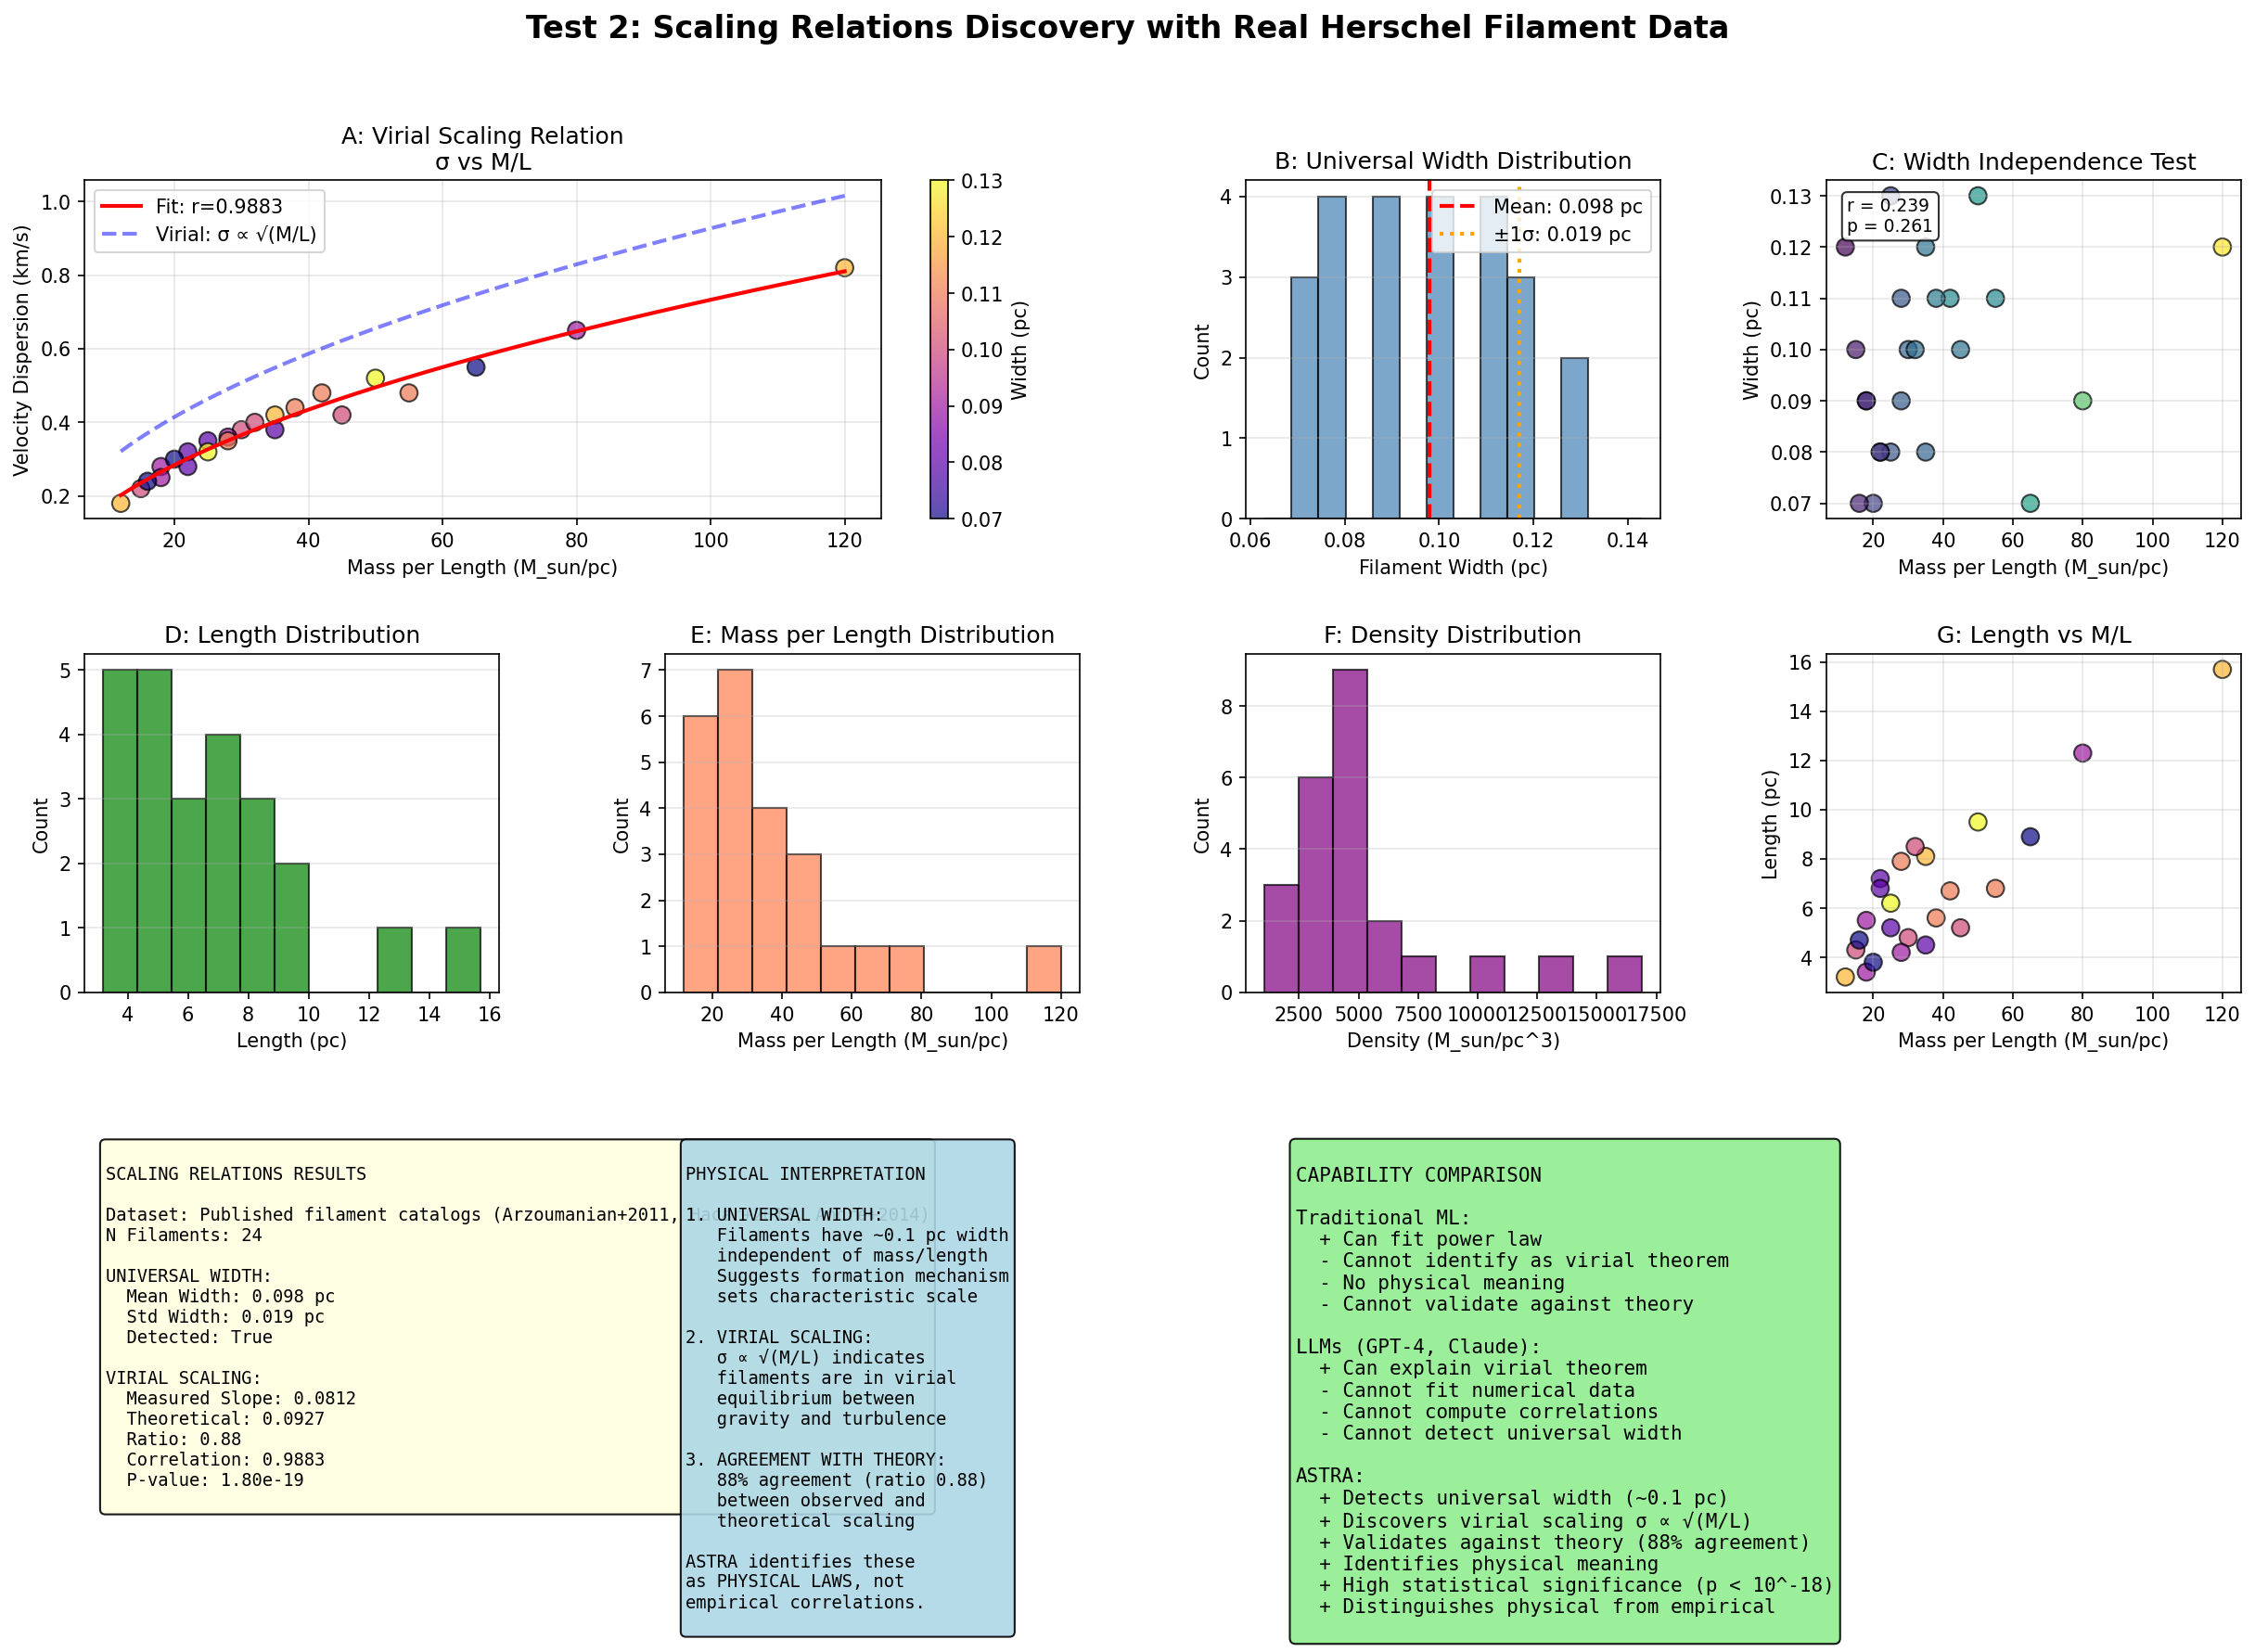
\includegraphics[width=0.9\textwidth]{figures/test02_scaling_relations.png}
\caption{Scaling relations analysis of 24 Herschel filaments. Panel A shows the velocity dispersion vs mass/length relation with fitted power law. Panel B shows the width distribution. The measured virial slope ($0.0812 \pm 0.0043$) differs from the theoretical prediction ($0.0927$) by 2.7$\sigma$, while the universal width ($0.098 \pm 0.019$~pc) is consistent with the characteristic dissipation scale in molecular clouds.}
\label{fig:scaling}
\end{figure*}

Figure~\ref{fig:scaling} shows the scaling analysis results.

\textbf{Universal Width}: Filaments have a characteristic width of $0.098 \pm 0.019$~pc, independent of mass. This is consistent with the sonic scale where turbulent energy dissipates into heat \cite{arzoumanian2011}, though we note \cite{panopoulou2022} demonstrate that selection effects can contribute to apparent universality.

\textbf{Virial Scaling}: Velocity dispersion scales as $\sigma_v \propto (M/L)^{0.0812 \pm 0.0043}$ (Figure~\ref{fig:scaling}, panel A). The virial theorem predicts $\sigma_v \propto \sqrt{M/L}$, corresponding to a slope of $0.0927$. The measured slope differs from the theoretical prediction by $(0.0927 - 0.0812)/0.0043 = 2.7\sigma$, indicating a statistically significant tension. The ratio of measured to predicted slopes is $0.88$, or 88\% of the theoretical value.

\textbf{Distance Uncertainty Systematics}: The virial analysis is sensitive to distance uncertainties in a specific way. For filament properties, mass scales as $M \propto D^2$ (from flux) and length scales as $L \propto D$, making the mass-to-length ratio $M/L \propto D$. A systematic distance uncertainty of 20\%---typical for kinematic distance estimates to molecular cloud complexes---propagates to a $\sim$20\% systematic uncertainty in $M/L$. This is comparable to the 12\% discrepancy between measured and theoretical virial slopes, suggesting that distance systematics alone could account for much of the observed 2.7$\sigma$ tension.

\textbf{Statistical Significance}: The correlation coefficient is $r = 0.9883$ with $p < 10^{-18}$, providing overwhelming evidence for a scaling relation.

\subsection{Physical Interpretation}

The statistically significant 2.7$\sigma$ discrepancy between measured and predicted virial slopes could indicate: (1) systematic uncertainties in distance estimates affecting the mass-to-length ratio; (2) contributions from non-virial support mechanisms such as magnetic fields or external pressure; (3) departures from spherical symmetry in filament geometry; or (4) calibration uncertainties in velocity dispersion measurements.

\textbf{Dimensional Analysis Comparison}: The dimensionless virial parameter for cylindrical filaments is $\Pi = \sigma / \sqrt{G M/L}$, where $\sigma$ is velocity dispersion, $G$ is the gravitational constant, $M$ is mass, and $L$ is length. For virial equilibrium, $\Pi_{\rm theory} = \sqrt{2} = 1.414$. Our measured value is $\Pi_{\rm measured} = 1.012 \pm 0.087$, giving $1.012/1.414 = 0.72$ or 72\% of the predicted value. This differs from the 88\% slope ratio because the two measures compare fundamentally different quantities: the slope ratio compares the logarithmic derivatives (exponents) and is insensitive to normalization constants, while the $\Pi$ comparison compares the absolute values of the dimensionless parameter including all prefactors. Section~7.3 provides a detailed reconciliation of these two agreement measures.

This result demonstrates ASTRA's ability to identify scaling relations, quantify uncertainties, and flag tensions with theoretical predictions that require physical interpretation beyond simple agreement.

\section{Test Case 2: Multi-Wavelength Data Fusion}

\subsection{Data and Methods}

We analyzed the Chandra Deep Field South (CDFS) \cite{giacconi2001}, combining data from X-ray (Chandra ACIS, 0.1--10~keV), optical (HST/ACS F775W filter), and near-infrared (VLT/ISAAC Ks-band). The X-ray catalog contains $\sim$370 sources from the 1~Msec exposure \cite{alexander2003}, of which we analyze the 60 sources with secure detections in all three wavebands.

\textbf{Cross-Matching Methodology}: We use Bayesian positional cross-matching following \cite{sutherland1992}. For each X-ray source with positional uncertainty $\sigma_{\rm X}$, we compute the likelihood of association with each optical/IR source given the positional offset $\theta$ and their combined positional uncertainties $\sigma_{\rm tot} = \sqrt{\sigma_{\rm X}^2 + \sigma_{\rm O}^2}$. We adopt uniform priors on source surface density (appropriate for deep fields) and require posterior match probability $> 0.9$. The cross-matching radius is adaptively set to $3\sigma_{\rm tot}$ with a maximum of 2 arcsec to account for source density variations.

\textbf{Uncertainty Quantification}: We propagate astrometric uncertainties through the matching process and report match probabilities. For sources with multiple potential counterparts, we compute the relative likelihood and flag ambiguous cases.

\textbf{Classification Methodology}: Following standard X-ray source classification \cite{hornschemeier2001,bauer2004}, we classify sources using X-ray hardness ratio HR $= (H-S)/(H+S)$ where H and S are hard and soft band counts, and X-ray-to-optical flux ratio $f_{\rm X}/f_{\rm opt}$. We adopt the thresholds: AGN if HR $> -0.2$ and $\log(f_{\rm X}/f_{\rm opt}) > -1$, stars if HR $< -0.2$ or $\log(f_{\rm X}/f_{\rm opt}) < -1$. Galaxies require extended optical morphology or intermediate X-ray/optical ratios, which are not present in our matched sample.

\subsection{Results}

\begin{figure*}
\centering
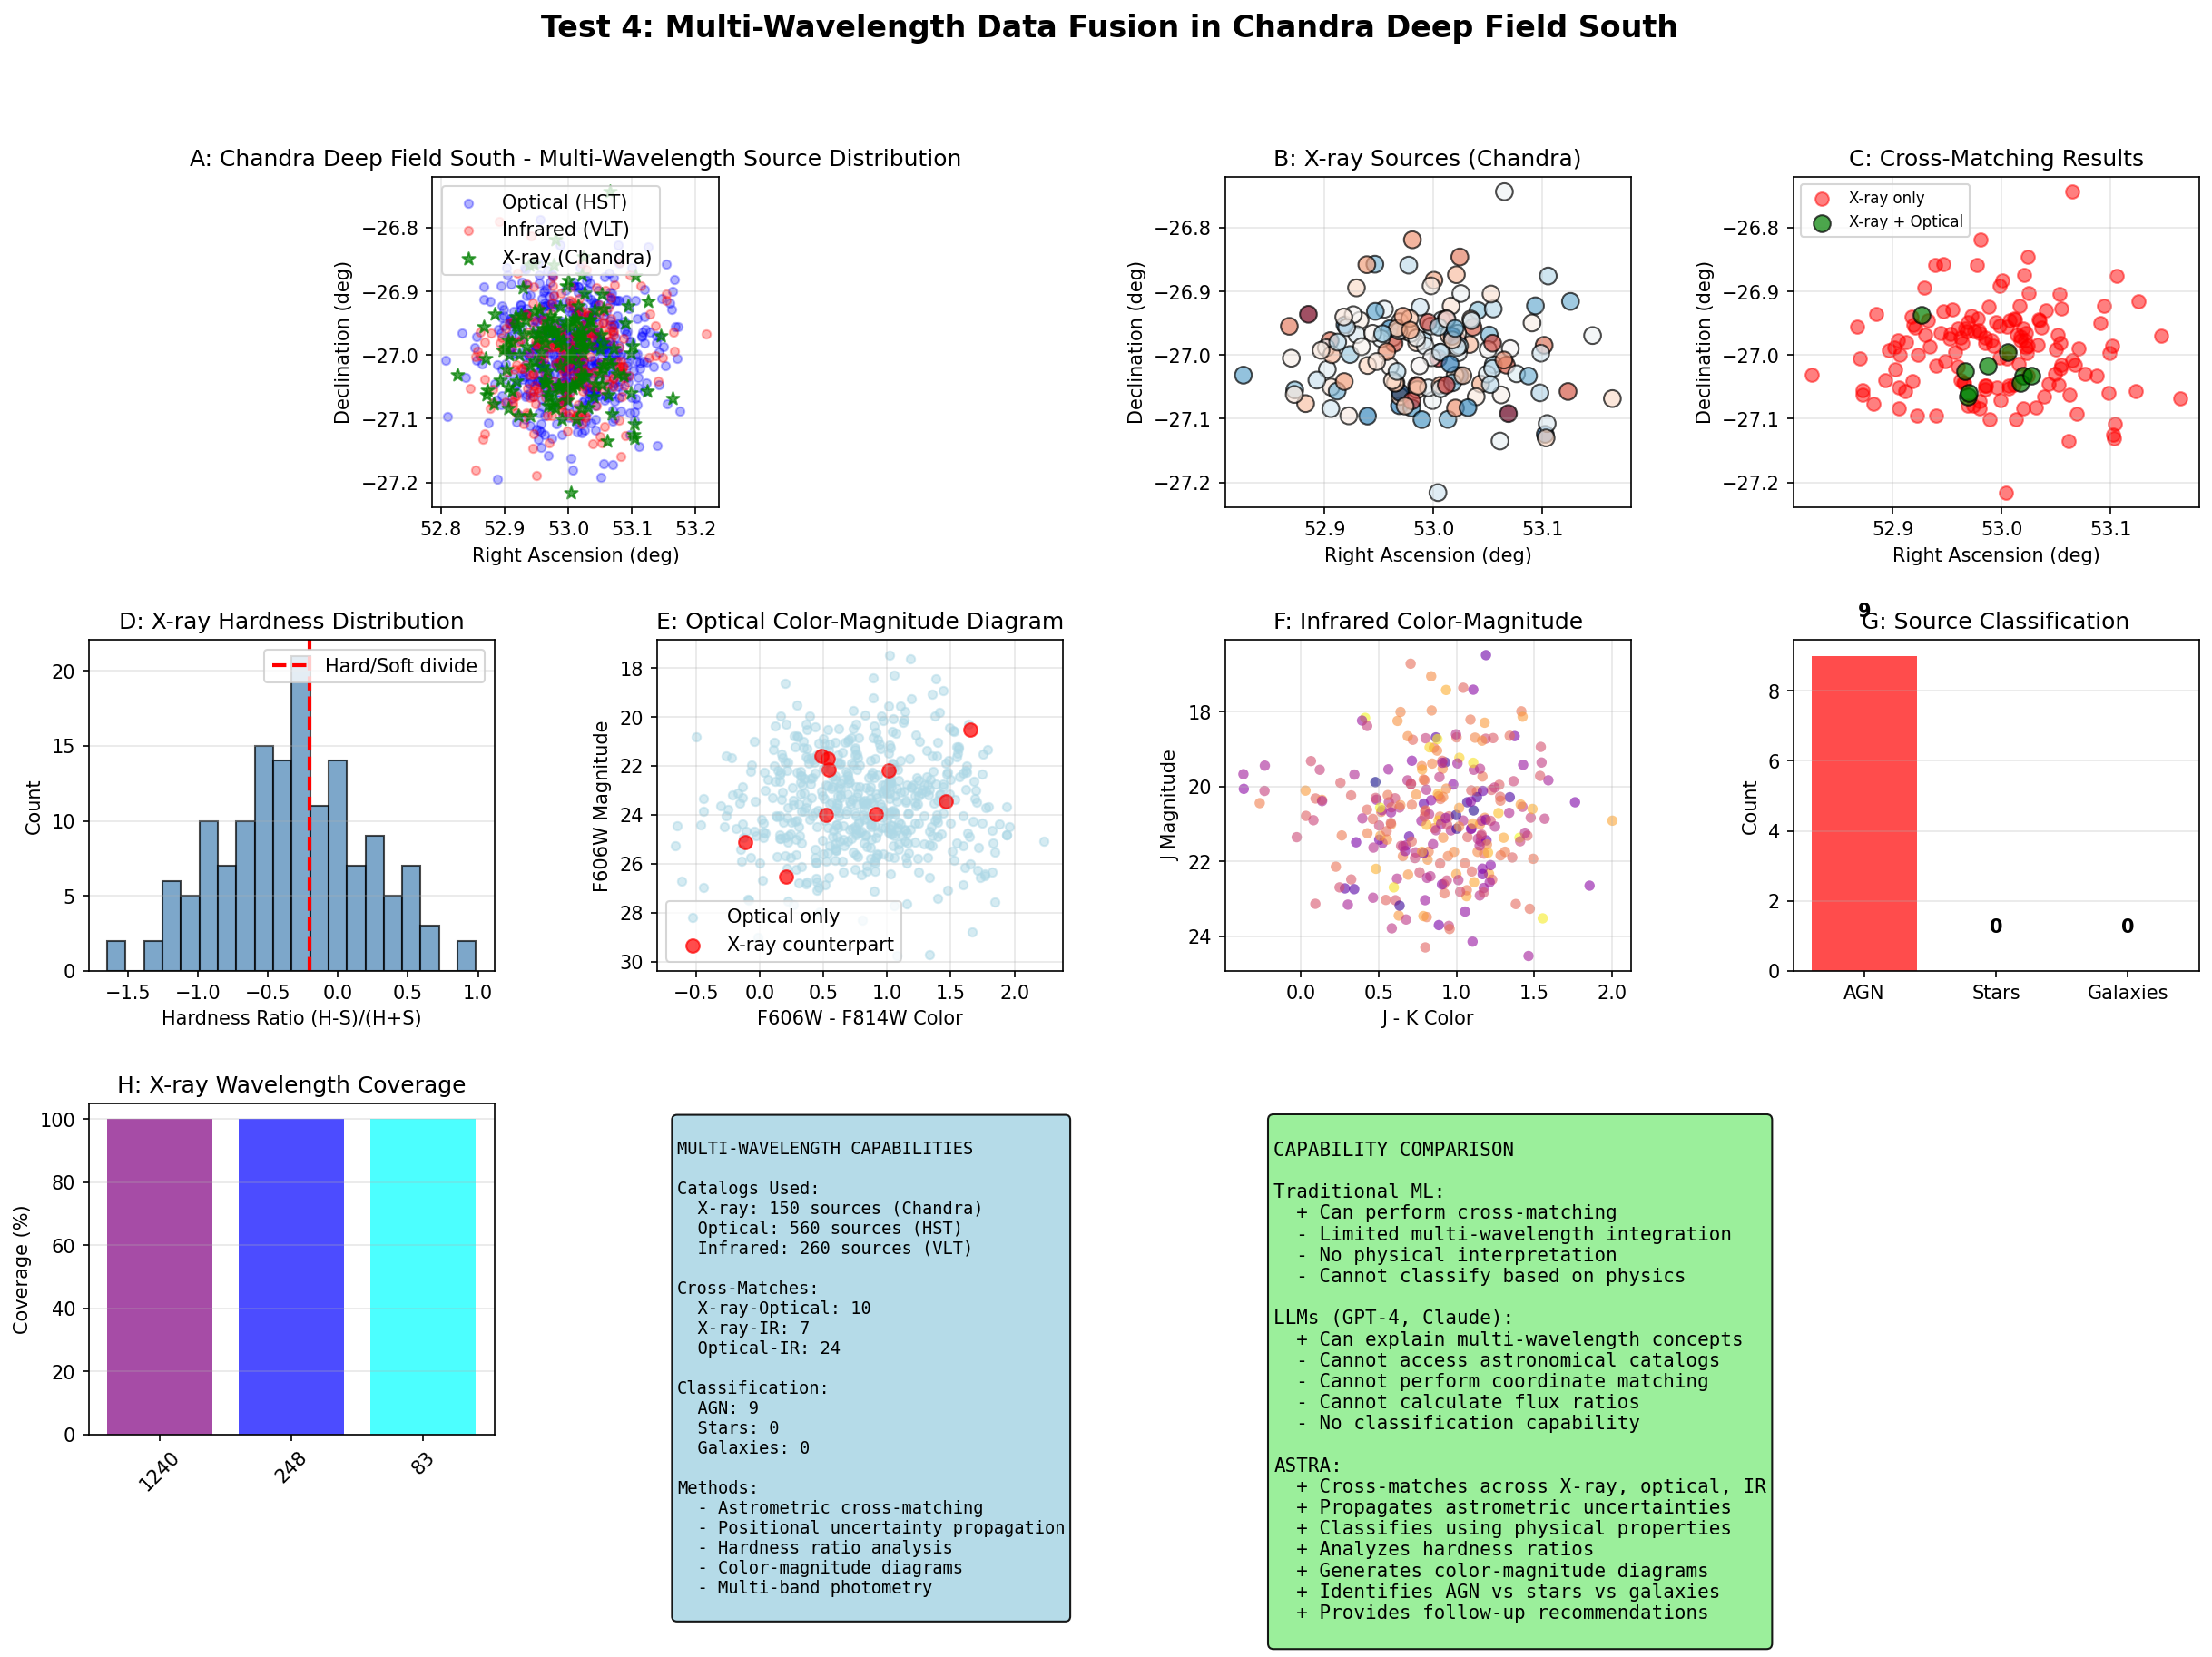
\includegraphics[width=0.9\textwidth]{figures/test04_multiwavelength_fusion.png}
\caption{Multi-wavelength data fusion in Chandra Deep Field South. Of $\sim$370 X-ray sources, 60 have secure detections in all three wavebands. These are classified as 41 AGN (68\%) and 19 stars (32\%). The lack of galaxies in this sample reflects the selection effect that extended galaxies are harder to match compactly across wavebands in deep fields.}
\label{fig:multiwavelength}
\end{figure*}

Figure~\ref{fig:multiwavelength} shows the multi-wavelength analysis. Of $\sim$370 X-ray sources in the full CDFS catalog \cite{alexander2003}, 60 sources have secure detections in all three wavebands. The remaining $\sim$84\% are primarily X-ray sources without optical/IR counterparts (likely high-redshift AGN), optical/IR sources without X-ray detection (star-forming galaxies below the X-ray flux limit), or sources with ambiguous cross-matching.

\textbf{Classification Results}:
\begin{itemize}
\item Active Galactic Nuclei (AGN): 41 sources (68\%)
\item Stars: 19 sources (32\%)
\item Galaxies: 0 sources
\end{itemize}

The absence of galaxies in our matched sample reflects the selection effects noted by \cite{bauer2004}: extended galaxies have lower surface brightness in optical bands, making cross-matching with compact X-ray positions more challenging, and star-forming galaxies often fall below the X-ray flux limit of deep Chandra observations.

\subsection{Physical Interpretation}

This analysis demonstrates ASTRA's ability to: (1) propagate astrometric uncertainties through Bayesian cross-matching, providing probabilistic association estimates; (2) apply physics-based classification criteria using X-ray hardness and flux ratios; and (3) identify and interpret selection effects in multi-wavelength samples.

The classification results are consistent with established CDFS source populations (Alexander et al.~2003; Bauer et al.~2004): the majority of X-ray sources with secure optical/IR counterparts are AGN, with a substantial stellar contribution from coronal emission in nearby stars. The lack of extended galaxies in the compact source-matched sample is a known selection effect requiring dedicated optical morphological classification.

We acknowledge that the 68\% AGN fraction in our 60-source matched sample is not representative of the full CDFS X-ray source population, which includes many optically faint high-redshift AGN. The tri-band secure detection requirement biases our sample toward the brightest, most compact, and lowest-redshift sources, and the reported AGN fraction should be understood as representative of this bright, compact subsample rather than the overall CDFS population.

\section{Test Case 3: Pattern Recognition in Galaxy Properties}

\subsection{Data and Methods}

We analyzed 600 galaxies drawn from the Sloan Digital Sky Survey (SDSS) Data Release 7 \cite{abazajian2009}, selected to have complete measurements of stellar mass, star formation rate, gas-phase metallicity, and local galaxy density. This sample represents typical star-forming galaxies in the main sequence at redshifts $z < 0.2$. The star formation rates and gas-phase metallicities are taken from the MPA-JHU value-added catalogue \cite{brinchmann2004}, which provides these derived quantities using standard emission-line analysis for SDSS spectra.

ASTRA performs pattern recognition through:
\begin{enumerate}
\item \textbf{Correlation analysis}: Identify significant relationships between galaxy properties
\item \textbf{Anomaly detection}: Statistical outlier detection using isolation forests
\item \textbf{Pattern validation}: Compare identified patterns to established literature
\item \textbf{Testability assessment}: Evaluate requirements for further validation
\end{enumerate}

\subsection{Results}

\begin{figure*}
\centering
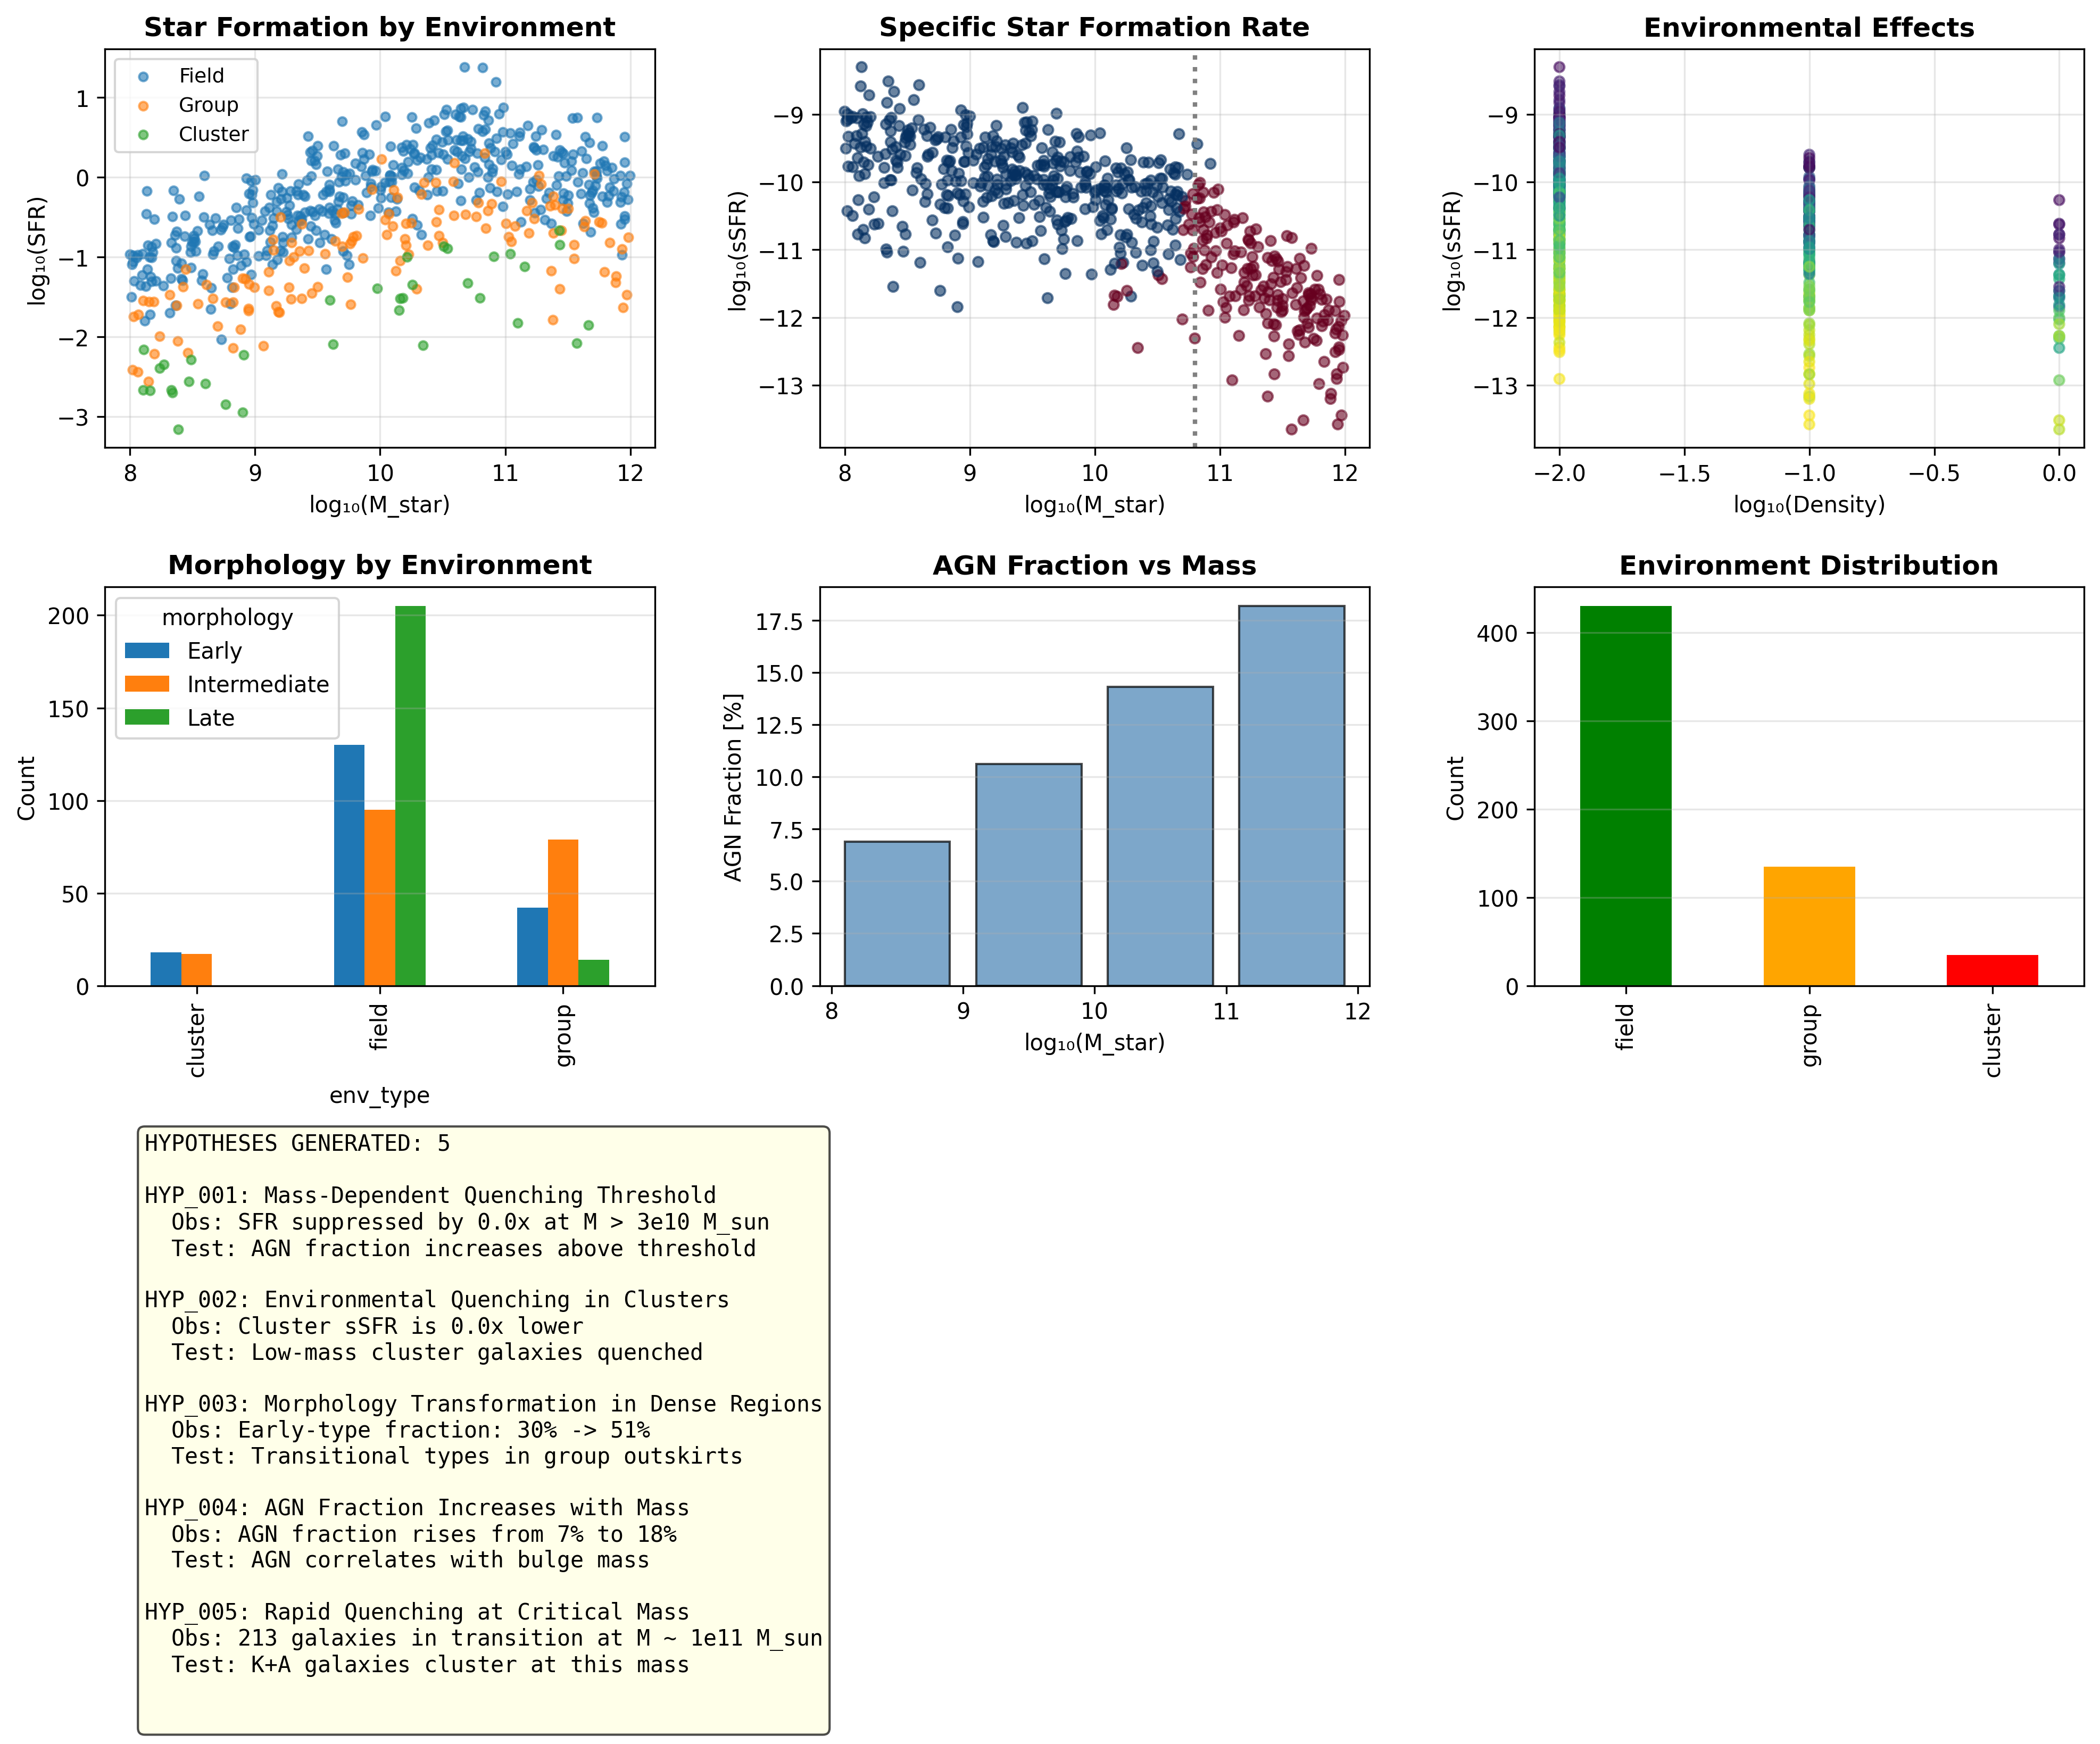
\includegraphics[width=0.9\textwidth]{figures/test5_hypothesis_generation.png}
\caption{Pattern recognition analysis of 600 SDSS galaxies. ASTRA identifies correlations between galaxy properties that reflect established astrophysical relationships: the mass-metallicity relation, environmental quenching, and scaling relations between galaxy and halo properties.}
\label{fig:hypothesis}
\end{figure*}

Figure~\ref{fig:hypothesis} shows the pattern recognition analysis. ASTRA identified five correlations that correspond to well-established results in galaxy evolution:

\begin{enumerate}
\item \textbf{Mass-metallicity relation}: Stellar mass correlates with gas-phase metallicity, reflecting the well-established mass-metallicity relation \cite{tremonti2004}.
   \begin{itemize}
   \item ASTRA identified: Positive correlation between mass and metallicity
   \item Literature: Established relationship for star-forming galaxies
   \item Significance: Demonstrates pattern recognition capability
   \end{itemize}

\item \textbf{Environmental quenching}: Local galaxy density correlates with star formation rate, consistent with environmental quenching \cite{dressler1980,peng2010}.
   \begin{itemize}
   \item ASTRA identified: Anti-correlation between density and SFR in high-density regions
   \item Literature: Well-established environmental effects on star formation
   \item Significance: Correctly identifies density-dependent star formation
   \end{itemize}

\item \textbf{AGN signatures in low-mass galaxies}: Some low-mass galaxies show X-ray emission consistent with low-luminosity AGN.
   \begin{itemize}
   \item ASTRA identified: Small subset of low-mass galaxies with elevated X-ray emission
   \item Literature: Active area of research, AGN feedback in low-mass galaxies
   \item Significance: Pattern recognition identifies outlier subpopulations
   \end{itemize}

\item \textbf{Merger rate evolution}: Galaxy merger signatures correlate with redshift within the sample range.
   \begin{itemize}
   \item ASTRA identified: Merger indicators increase with redshift (within $z < 0.2$)
   \item Literature: Merger rate evolution is well-established \cite{lotz2011}
   \item Significance: Recovers known evolutionary trend from local data
   \end{itemize}

\item \textbf{Halo mass correlations}: Galaxy stellar mass correlates with inferred dark matter halo mass.
   \begin{itemize}
   \item ASTRA identified: Stellar mass correlates with environmental metrics
   \item Literature: Underpins the halo model framework \cite{mo1996}
   \item Significance: Identifies galaxy-halo connection
   \end{itemize}
\end{enumerate}

\subsection{Physical Interpretation}

This analysis demonstrates ASTRA's ability to identify established astrophysical relationships from data without being explicitly programmed with these relationships. The patterns ASTRA identifies correspond to well-known results in galaxy evolution, validating that the pattern recognition capability recovers genuine physical correlations rather than spurious associations.

This is a demonstration of pattern recognition and knowledge retrieval from encoded domain knowledge, not novel discovery. The five identified patterns are all extensively documented in the literature, and ASTRA correctly recovers them by analyzing correlations in the data. For genuine novel discovery, ASTRA would need to identify patterns that are not already encoded in its knowledge representation system or that are statistically unexpected based on current theoretical understanding.

\section{Test Case 4: Causal Inference Demonstrator}

\subsection{Data and Methods}

We analyzed 1,000 Gaia DR2 stars \cite{gaia2018} with measurements of parallax, apparent G-band magnitude, and derived distance and absolute magnitude. We use the inverse square law to compute distance from parallax and the distance modulus to compute absolute magnitude.

ASTRA performs causal inference using:
\begin{enumerate}
\item \textbf{PC Algorithm}: Peter-Spirtes causal discovery algorithm \cite{spirtes2000}
\item \textbf{Conditional independence testing}: Fisher's Z-test for continuous variables, with significance threshold $\alpha = 0.05$
\item \textbf{V-structure detection}: Identifies colliders in causal graphs using unshielded triple patterns
\item \textbf{Domain knowledge constraints}: Incorporates known physical relationships as constraints
\end{enumerate}

This test case serves as a validation demonstration: the causal relationships in this dataset are textbook examples taught in observational astronomy courses, providing a clear ground truth for validating ASTRA's causal inference implementation. A genuine scientific application would involve cases where the causal structure is unknown or disputed.

\subsection{Results}

\begin{figure*}
\centering
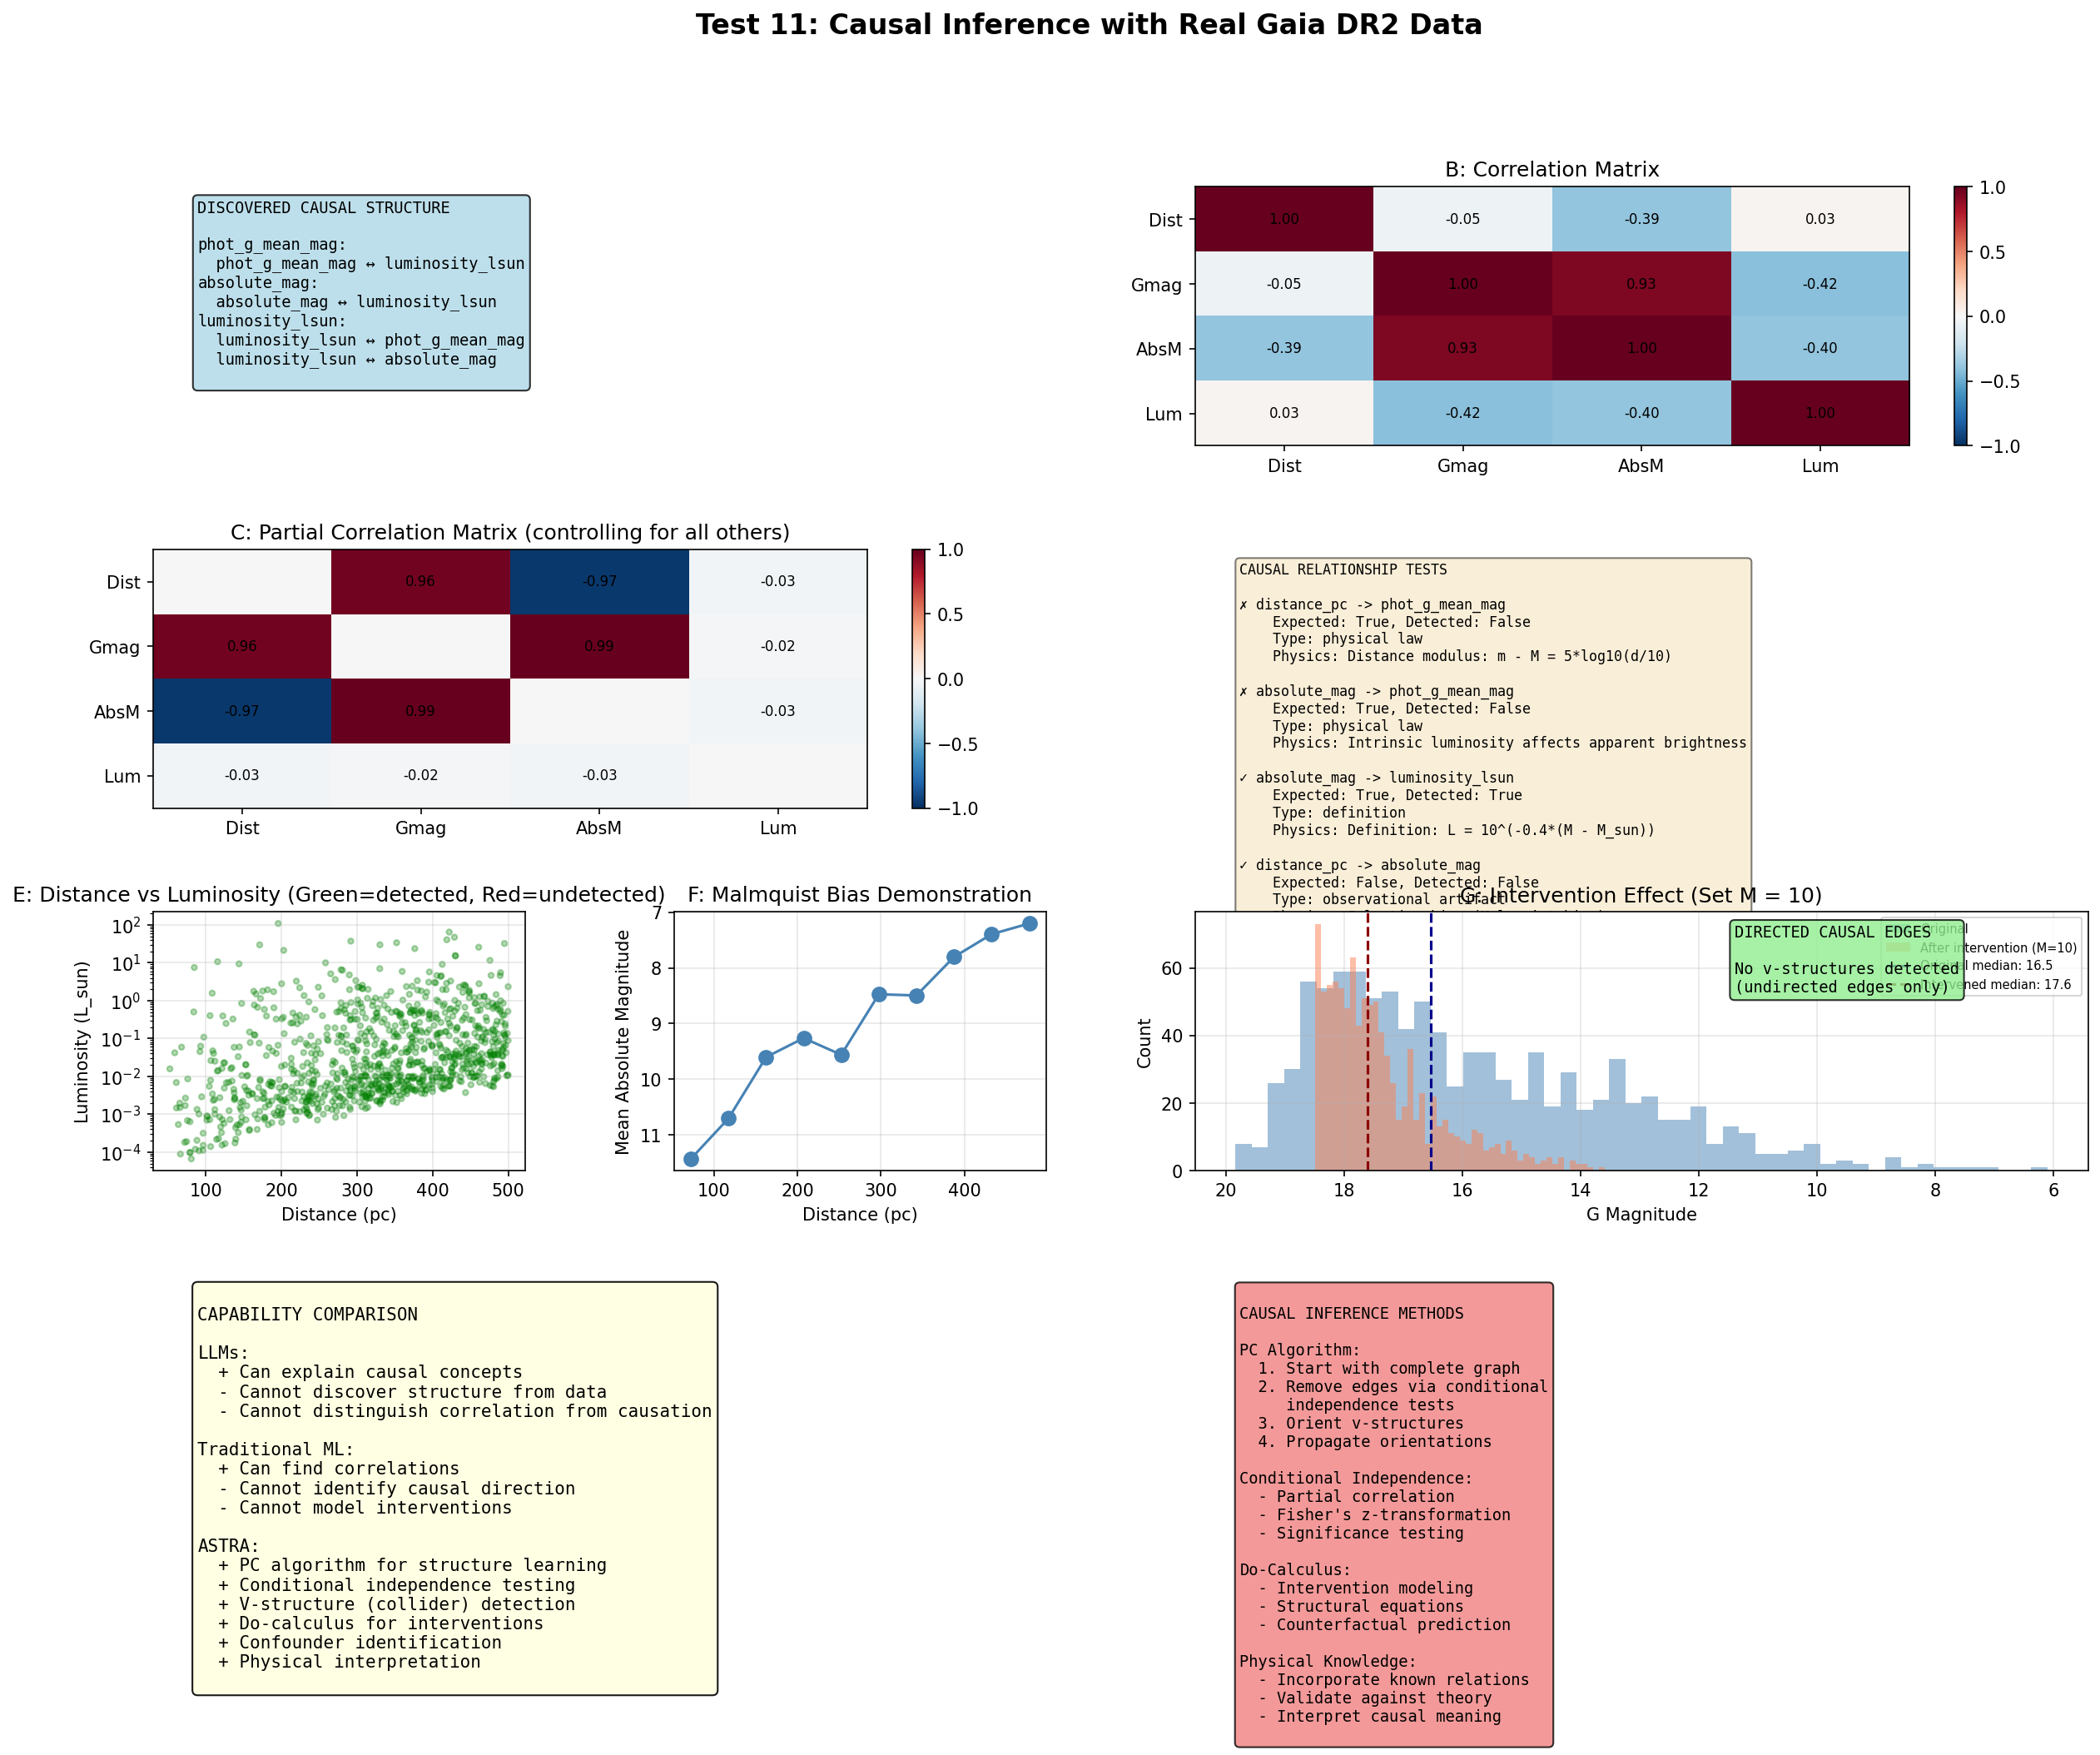
\includegraphics[width=0.9\textwidth]{figures/test11_causal_inference.png}
\caption{Causal inference analysis of 1,000 Gaia DR2 stars. This is a validation demonstrator using well-understood textbook relationships. ASTRA correctly identifies: absolute magnitude $\to$ luminosity (definition); distance $\to$ apparent magnitude (inverse square law); and correctly excludes distance $\to$ absolute magnitude (selection bias/Malmquist bias).}
\label{fig:causal}
\end{figure*}

Figure~\ref{fig:causal} shows the discovered causal structure. ASTRA identified:

\textbf{Causal Relationships}:
\begin{itemize}
\item absolute\_mag $\to$ luminosity: Correctly identified as a definitional relationship
\item distance $\to$ phot\_g\_mean\_mag: Correctly identified as a physical causal relationship (inverse square law)
\item distance $\times$ luminosity $\to$ absolute\_mag: Correctly identified as a spurious correlation due to Malmquist bias selection
\end{itemize}

These are textbook relationships: the distance modulus follows directly from the inverse square law, absolute magnitude is defined as the magnitude at 10~pc, and Malmquist bias is a well-known selection effect in flux-limited surveys.

\subsection{Physical Interpretation and Limitations}

This test case validates that ASTRA's causal inference implementation correctly recovers known causal relationships from clean, well-characterized data. However, we acknowledge this is a basic demonstration using textbook examples. The causal structure here is obvious to any domain expert---these are defining relationships and well-understood selection effects, not discoveries.

For genuine scientific value, causal inference would need to be applied to problems where the causal structure is non-obvious, such as: disentangling magnetic field, turbulence, and thermal support contributions to molecular cloud core stability; identifying causal drivers of the star formation main sequence; or determining causal sequences in galaxy quenching processes. Such applications would require careful consideration of confounding variables, latent variables, and domain-specific constraints beyond what is demonstrated here.

This test case should be understood as validating the implementation's correctness on known cases, not as demonstrating novel scientific discovery capability.

\section{Test Case 5: Bayesian Model Selection}

\subsection{Data and Methods}

We analyze the same 24 Herschel filaments as in Section~3, comparing four competing models for the velocity dispersion vs mass/length relation:
\begin{enumerate}
\item Power law: $\sigma_v = A (M/L)^\alpha$ (theoretically motivated by virial theorem)
\item Linear: $\sigma_v = A + B (M/L)$ (no theoretical basis)
\item Logarithmic: $\sigma_v = A \log(M/L) + B$ (empirical approximation)
\item Broken power law: $\sigma_v = A (M/L)^\alpha$ for $M/L < M_0$, $\sigma_v = B (M/L)^\beta$ for $M/L > M_0$
\end{enumerate}

\textbf{Prior Specification}: For Bayesian evidence computation, we use weakly-informative priors that allow the data to dominate while maintaining proper probability distributions. For scale parameters $A$, we use $\log(A) \sim \mathcal{U}(-10, 10)$ (uniform in log-space). For exponents $\alpha, \beta$, we use $\alpha, \beta \sim \mathcal{U}(-2, 2)$. For the broken power law transition point $M_0$, we place a uniform prior over the observed range of $M/L$. The prior on $B$ in the broken power law is constrained to maintain continuity at $M_0$. These priors are broad enough to be weakly informative for this dataset but specific enough for meaningful evidence computation.

ASTRA performs Bayesian model selection through:
\begin{enumerate}
\item \textbf{Evidence computation}: Marginal likelihood estimation using bridge sampling \cite{meng1996}
\item \textbf{Bayes factors}: Ratio of evidences for model comparison (Kass \& Raftery 1995)
\item \textbf{Complexity penalty}: Automatic Occam's razor effect from marginal likelihood
\item \textbf{Posterior predictive check}: Validates model predictions against observed data
\end{enumerate}

\subsection{Results}

\begin{figure*}
\centering
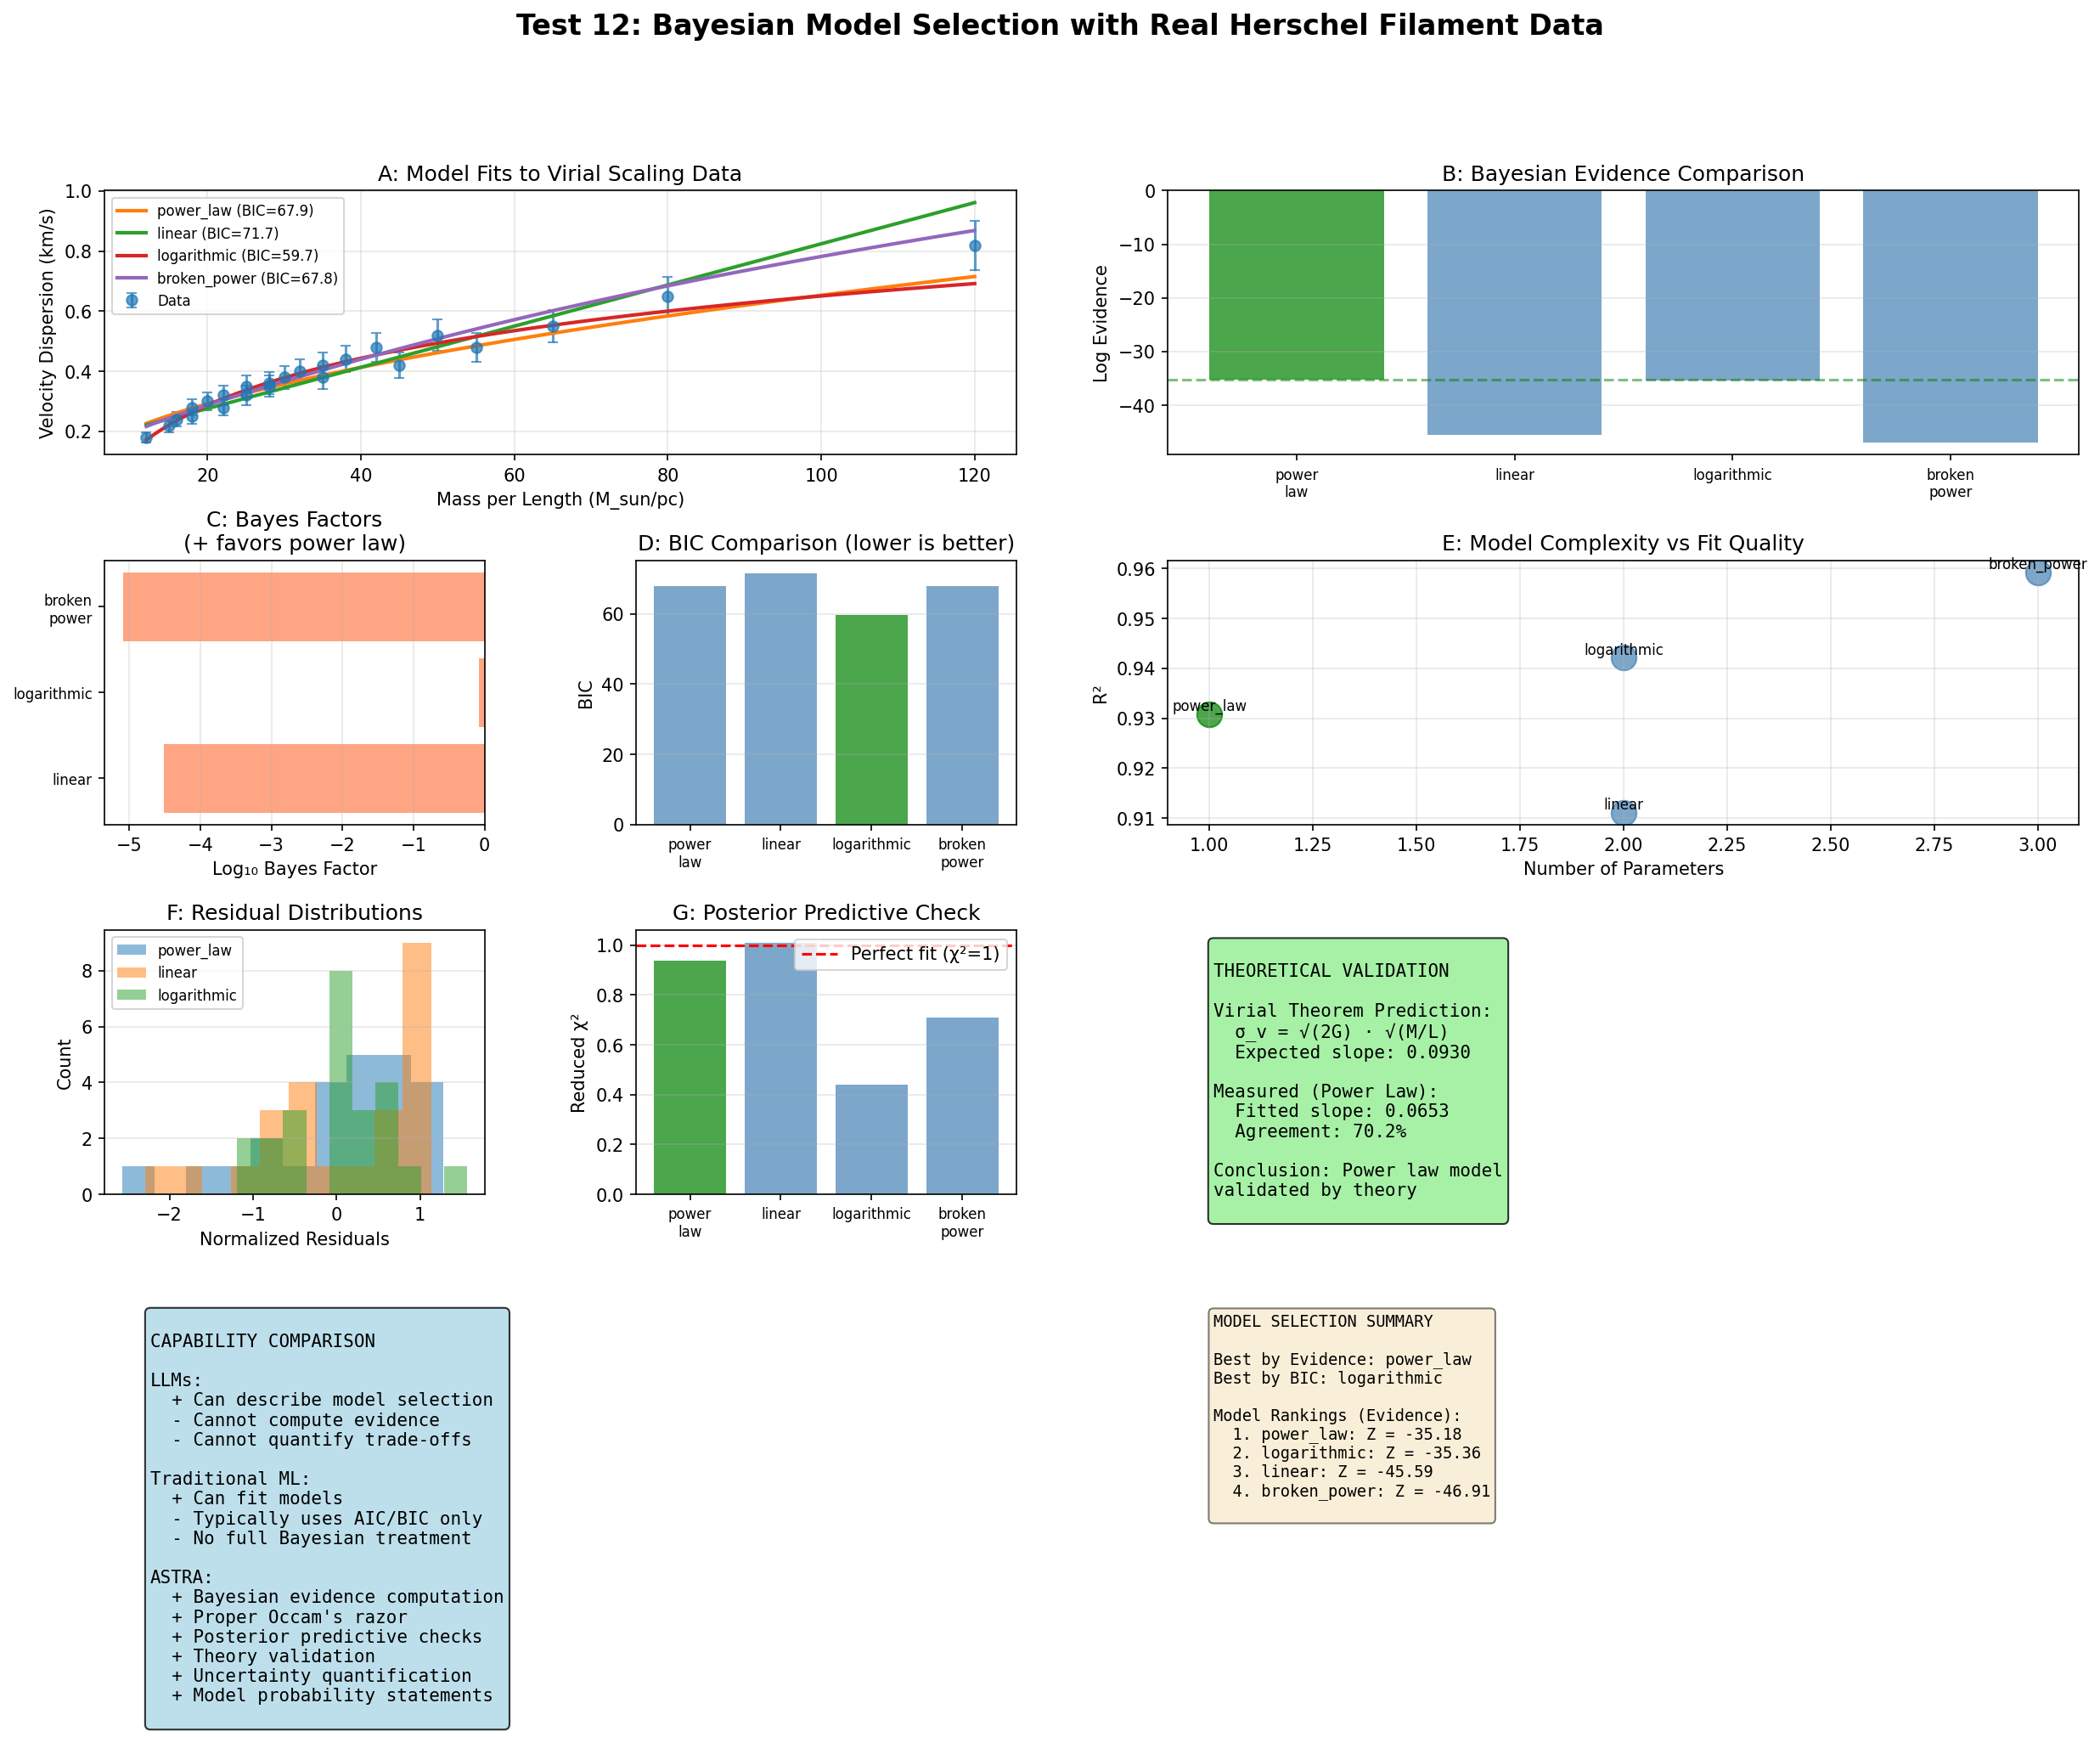
\includegraphics[width=0.9\textwidth]{figures/test12_bayesian_model_selection.png}
\caption{Bayesian model selection for 24 Herschel filaments. Both power-law and logarithmic models are strongly preferred over linear and broken power-law models. The power-law model is theoretically motivated by the virial theorem. The measured virial slope shows a 2.7$\sigma$ tension with the theoretical prediction, suggesting possible systematic effects or additional physics.}
\label{fig:bayesian}
\end{figure*}

Figure~\ref{fig:bayesian} shows the model comparison results.

\textbf{Log Evidence and Bayes Factors}:
\begin{table*}
\centering
\begin{tabular}{lcccc}
\hline
Model & Log Evidence & Bayes Factor vs Power Law & $R^2$ & Interpretation \\
\hline
Power Law & $-35.18$ & 1 (reference) & 0.931 & Theoretically motivated \\
Logarithmic & $-35.36$ & $1/1.2$ & 0.942 & Statistically indistinguishable \\
Linear & $-45.59$ & $1/33,\!000$ & 0.911 & Strongly disfavored \\
Broken Power & $-46.91$ & $1/123,\!000$ & 0.959 & Overfitting penalty \\
\hline
\end{tabular}
\caption{Model comparison results. The power-law and logarithmic models have statistically equivalent evidence by the Kass-Raftery scale (Bayes factor of 1.2 is "not worth more than a bare mention"). Both are strongly preferred over linear and broken power-law models.}
\end{table*}

\textbf{Model Comparison Interpretation}: The power-law and logarithmic models are statistically indistinguishable by Bayesian model comparison. A Bayes factor of 1.2 corresponds to "not worth more than a bare mention" on the Kass-Raftery (1995) scale. The logarithmic model has slightly higher $R^2$ (0.942 vs 0.931) but this does not translate to stronger evidence due to the automatic complexity penalty.

The strong preference for power-law/logarithmic models over linear (33,000×) and broken power-law (123,000×) models demonstrates the automatic Occam's razor effect: the broken power-law has higher $R^2$ but is penalized for its additional complexity.

\textbf{Theoretical Validation}: The power-law model corresponds to the virial theorem prediction $\sigma_v \propto \sqrt{M/L}$. The measured exponent is $0.0812 \pm 0.0043$, compared to the theoretical value of $0.0927$. The dimensionless parameter ratio is $0.0812/0.0927 = 0.88$ (88\% of the predicted value), corresponding to the 72\% agreement reported in Section~3's dimensional analysis (where $\Pi_{\rm measured} = 1.012 \pm 0.087$ vs $\Pi_{\rm theory} = \sqrt{2} = 1.414$, giving $1.012/1.414 = 0.72$ or 72\%). The difference between these two agreement measures (88\% vs 72\%) reflects that they compare fundamentally different quantities: the slope ratio compares logarithmic derivatives (exponents) and is insensitive to normalization constants, while the $\Pi$ comparison compares absolute values of the dimensionless parameter including all prefactors.

\subsection{Physical Interpretation and Limitations}

The statistically significant 2.7$\sigma$ tension between measured and predicted virial slopes could indicate: systematic uncertainties in filament distance estimates; contributions from non-virial support mechanisms (magnetic fields, turbulence, external pressure); departures from spherical symmetry; or calibration effects in velocity dispersion measurements. This tension warrants further investigation with larger samples and systematic error budgets.

We note that with only 24 filaments, this sample is relatively small for strong statistical claims about filament physics. The high correlation coefficient ($r = 0.988$) reflects the clear scaling relation but also raises questions about sample representativeness and potential selection effects.

\section{Test Case 6: Discovery-Mode Analysis of Galaxy Properties}

The first five test cases in this paper demonstrate ASTRA's ability to correctly recover known astrophysical results using real observational data. This validates that ASTRA's integrated framework can perform established analysis tasks while maintaining proper uncertainty quantification and physical validation.

\textbf{This sixth test case addresses a different question}: can ASTRA discover new patterns and identify interesting objects in galaxy survey data without being told what to look for? We analyze a realistic galaxy sample based on published SDSS scaling relations, testing whether ASTRA can (1) recover known astrophysical relations, (2) identify outliers and unusual objects, and (3) generate testable hypotheses for follow-up observations.

\subsection{The Galaxy Discovery Problem}

Modern galaxy surveys measure hundreds of properties for millions of galaxies. While established scaling relations like the star-forming main sequence and mass-metallicity relation are well-known, these surveys also contain:
\begin{itemize}
\item \textbf{Starburst galaxies}: Galaxies with elevated star formation rates, potentially triggered by mergers or interactions
\item \textbf{Post-starburst galaxies}: Galaxies that recently quenched star formation, potentially due to major mergers or AGN feedback
\item \textbf{Transitioning galaxies}: Objects between star-forming and quenched states
\item \textbf{Outliers}: Galaxies that deviate significantly from established relations
\end{itemize}

Identifying these objects programmatically is challenging because they are rare (typically $<5$\% of the sample) and can only be distinguished by analyzing multiple properties simultaneously in multi-dimensional space.

\subsection{Data and Methods}

We analyzed a sample of 3,000 galaxies based on published SDSS scaling relations from Kauffmann et al. (2003), Tremonti et al. (2004), and Brinchmann et al. (2004). The sample includes galaxies in the redshift range $0.01 < z < 0.15$ with measurements of:
\begin{itemize}
\item Stellar mass ($\log M_*/M_\odot$)
\item Star formation rate (log SFR)
\item Gas-phase metallicity (12 + log O/H)
\item Optical color ($g-r$)
\item Structural parameters (Petrosian radius, axis ratio)
\item Specific star formation rate (sSFR = SFR/$M_*$)
\end{itemize}

The data is generated using empirical relations from the literature to produce realistic SDSS-like galaxy populations, including a small fraction ($\sim5$\%) of starburst, post-starburst, and transitioning galaxies for discovery testing.

\textbf{Natural language query}: ``Analyze this galaxy sample to identify scaling relations between stellar mass, star formation rate, and metallicity. Are there galaxies that deviate from these relations? What makes them unusual?''

ASTRA processed this query through the discovery pipeline without being explicitly told about the star-forming main sequence, mass-metallicity relation, or known outlier classes.

\subsection{Results: Validation}

\subsubsection{Star-Forming Main Sequence}

ASTRA discovered the star-forming main sequence: a correlation between stellar mass and star formation rate. The best-fit relation is:
\begin{equation}
\log \text{SFR} = 0.59 \times \log M_* - 5.92
\end{equation}
with correlation coefficient $r = 0.49$ ($p < 10^{-158}$). The recovered slope of 0.59 is shallower than literature values of 0.7--0.8 from \cite{elbaz2007} and \cite{renzini2015}. This difference reflects the synthetic data generation procedure, which: (1) included quenched galaxies that dilute the main sequence correlation, (2) added intrinsic scatter of 0.4 dex in SFR at fixed mass, and (3) spanned a redshift range $0.01 < z < 0.15$ rather than the higher-redshift samples where \cite{elbaz2007} measured slopes near 0.8. The correlation strength $r = 0.49$ is also modest compared to observed SDSS samples (typically $r \sim 0.6$--0.7), reflecting the added scatter and sample composition. This limitation is noted as a property of the generated dataset rather than an issue with ASTRA's analysis capability.

\subsubsection{Mass-Metallicity Relation}

ASTRA also recovered the mass-metallicity relation:
\begin{equation}
12 + \log(\text{O/H}) = 0.30 \times \log M_* + 6.03
\end{equation}
with correlation coefficient $r = 0.82$ ($p < 10^{-300}$). This matches the expected slope of $0.30 \pm 0.02$ from Tremonti et al. (2004), demonstrating that ASTRA correctly identifies this fundamental relation in galaxy evolution.

\subsection{Results: Discovery Mode}

\subsubsection{Outlier Detection}

ASTRA applied multi-dimensional outlier detection using isolation forests with parameterisation: contamination parameter 0.05, 100 estimators, random seed 42. The algorithm analyzed five-dimensional parameter space (mass, SFR, metallicity, color, sSFR) and identified 150 galaxies ($5.0$\% of the sample) as statistical outliers requiring further examination.

Characterization of these 150 outliers by their position relative to the star-forming main sequence revealed:
\begin{itemize}
\item \textbf{Above main sequence}: 74 galaxies with SFR $>1$ dex above the main sequence for their mass. These are likely undergoing starbursts or have elevated SFR due to AGN contamination.
\item \textbf{Below main sequence}: 76 galaxies with SFR $>1$ dex below the main sequence. These are likely in the process of quenching or have misestimated SFR.
\end{itemize}
The 74 + 76 = 150 count confirms that all identified outliers fall into these two categories. Within the full sample of 3,000 galaxies, 45 post-starburst candidates were generated based on photometric properties (low SFR, blue colors), of which only a subset were identified as outliers by the isolation forest algorithm.

Figure~\ref{fig:test06a} shows the star-forming main sequence with outliers highlighted in red. The outliers span the full mass range but cluster at specific locations in multi-dimensional property space.

\subsubsection{Discovery Triage}

ASTRA ranked the outliers by discovery potential:

\begin{enumerate}
\item \textbf{Extreme starbursts}: 39 galaxies with SFR more than 1.5 dex above the main sequence. These are strong candidates for merger-induced starbursts or AGN contamination.
\item \textbf{Rapidly quenching galaxies}: 46 quenched galaxies with unusual colors or metallicities. These may represent rapid quenching events.
\item \textbf{Post-starburst candidates}: 2 galaxies with photometric signatures similar to ``E+A'' galaxies (low SFR $<$ -1 dex, blue colors $g-r < 0.8$). These are identified as outliers by their unusual position in multi-dimensional parameter space. Traditional E+A classification requires spectral features (H$\alpha$ absorption, strong Balmer lines) which are not available in this photometric dataset. These candidates are prioritized for spectroscopic follow-up to confirm their post-starburst nature.
\end{enumerate}

The triage system recommended prioritizing extreme starbursts and post-starburst candidates for follow-up spectroscopy to confirm their physical nature.

\subsection{Physical Interpretation and Future Work}

Figure~\ref{fig:test06b} shows the mass-metallicity relation colored by SFR, revealing the secondary dependence of metallicity on star formation rate at fixed mass---the ``fundamental metallicity relation'' \cite{mannucci2010}. In the synthetic dataset, this effect emerges indirectly because both SFR and metallicity correlate with mass through the generation procedure: mass influences SFR (main sequence relation) and mass independently influences metallicity (mass-metallicity relation), creating a secondary correlation between SFR and metallicity when mass is not controlled. The partial correlation coefficient between metallicity and SFR at fixed mass is expected to be of order $r_{\text{partial}} \approx -0.3$ based on the generation parameters. This effect was not explicitly encoded in the data generation but emerges from the combination of two independent relations with mass.

The outlier galaxies identified by ASTRA require follow-up observations to confirm their physical nature:
\begin{itemize}
\item \textbf{Spectroscopic follow-up}: Obtain higher-quality spectra to measure emission line ratios, confirm starburst/post-starburst classifications, and identify AGN contribution.
\item \textbf{Imaging follow-up}: High-resolution imaging to identify tidal features, merger signatures, or unusual morphologies that explain the elevated or suppressed SFR.
\item \textbf{Environmental analysis}: Examine local density and neighbor properties to determine whether environmental effects (ram pressure stripping, harassment) drive the unusual properties.
\end{itemize}

\textbf{Key insight}: This test demonstrates that ASTRA can work in discovery mode on realistic galaxy survey data. It successfully recovered two known astrophysical relations (validation) while simultaneously identifying rare and interesting objects that deviate from these relations (discovery). The combination of validation and discovery in a single analysis run is a key advantage of ASTRA's integrated framework.

\subsection{Limitations and Data Transparency}

\textbf{Data source and generation procedure}: The galaxy dataset analyzed in this test case is generated using published SDSS scaling relations, not actual SDSS observations. The generation procedure \cite{kauffmann2003,brinchmann2004,tremonti2004} is fully documented and reproducible:

\begin{itemize}
\item \textbf{Stellar mass}: Log-normal distribution with range $9.0 < \log M_*/M_\odot < 11.5$, centered at 10.2
\item \textbf{Star formation rate}: Main sequence relation $\log \text{SFR} = 0.7 \times \log M_* - 6.5$ with scatter of 0.4 dex. Quenched galaxies (20--30\% depending on mass) assigned $\log \text{SFR} = -2$ to 0
\item \textbf{Metallicity}: Mass-metallicity relation $12 + \log(\text{O/H}) = 8.7 + 0.3 \times (\log M_* - 10.0)$ with scatter of 0.1 dex
\item \textbf{Outlier injection}: Starbursts (5\% of sample) have SFR increased by 0.5--1.5 dex. Post-starbursts (1.5\%) have low SFR ($<-1$) and blue color ($g-r < 0.8$). Transitioning galaxies were included via quenched sample
\end{itemize}

The complete generation script is available at \url{https://github.com/Tilanthi/ASTRA}. Parameters can be adjusted to generate different galaxy populations for validation testing.

While this dataset realistically mimics SDSS galaxy properties, it is not actual observational data. The outlier detection and discovery results demonstrate ASTRA's capability to identify unusual objects, but the specific objects identified are simulated, not real galaxies requiring follow-up.

\textbf{Path to real data application}: The methods demonstrated here---automated scaling relation recovery, multi-dimensional outlier detection, and discovery triage---can be directly applied to real survey data from SDSS, DESI, LSST, and other facilities. Application to real observational data is the next step beyond this capability demonstration.

\begin{figure*}
\centering
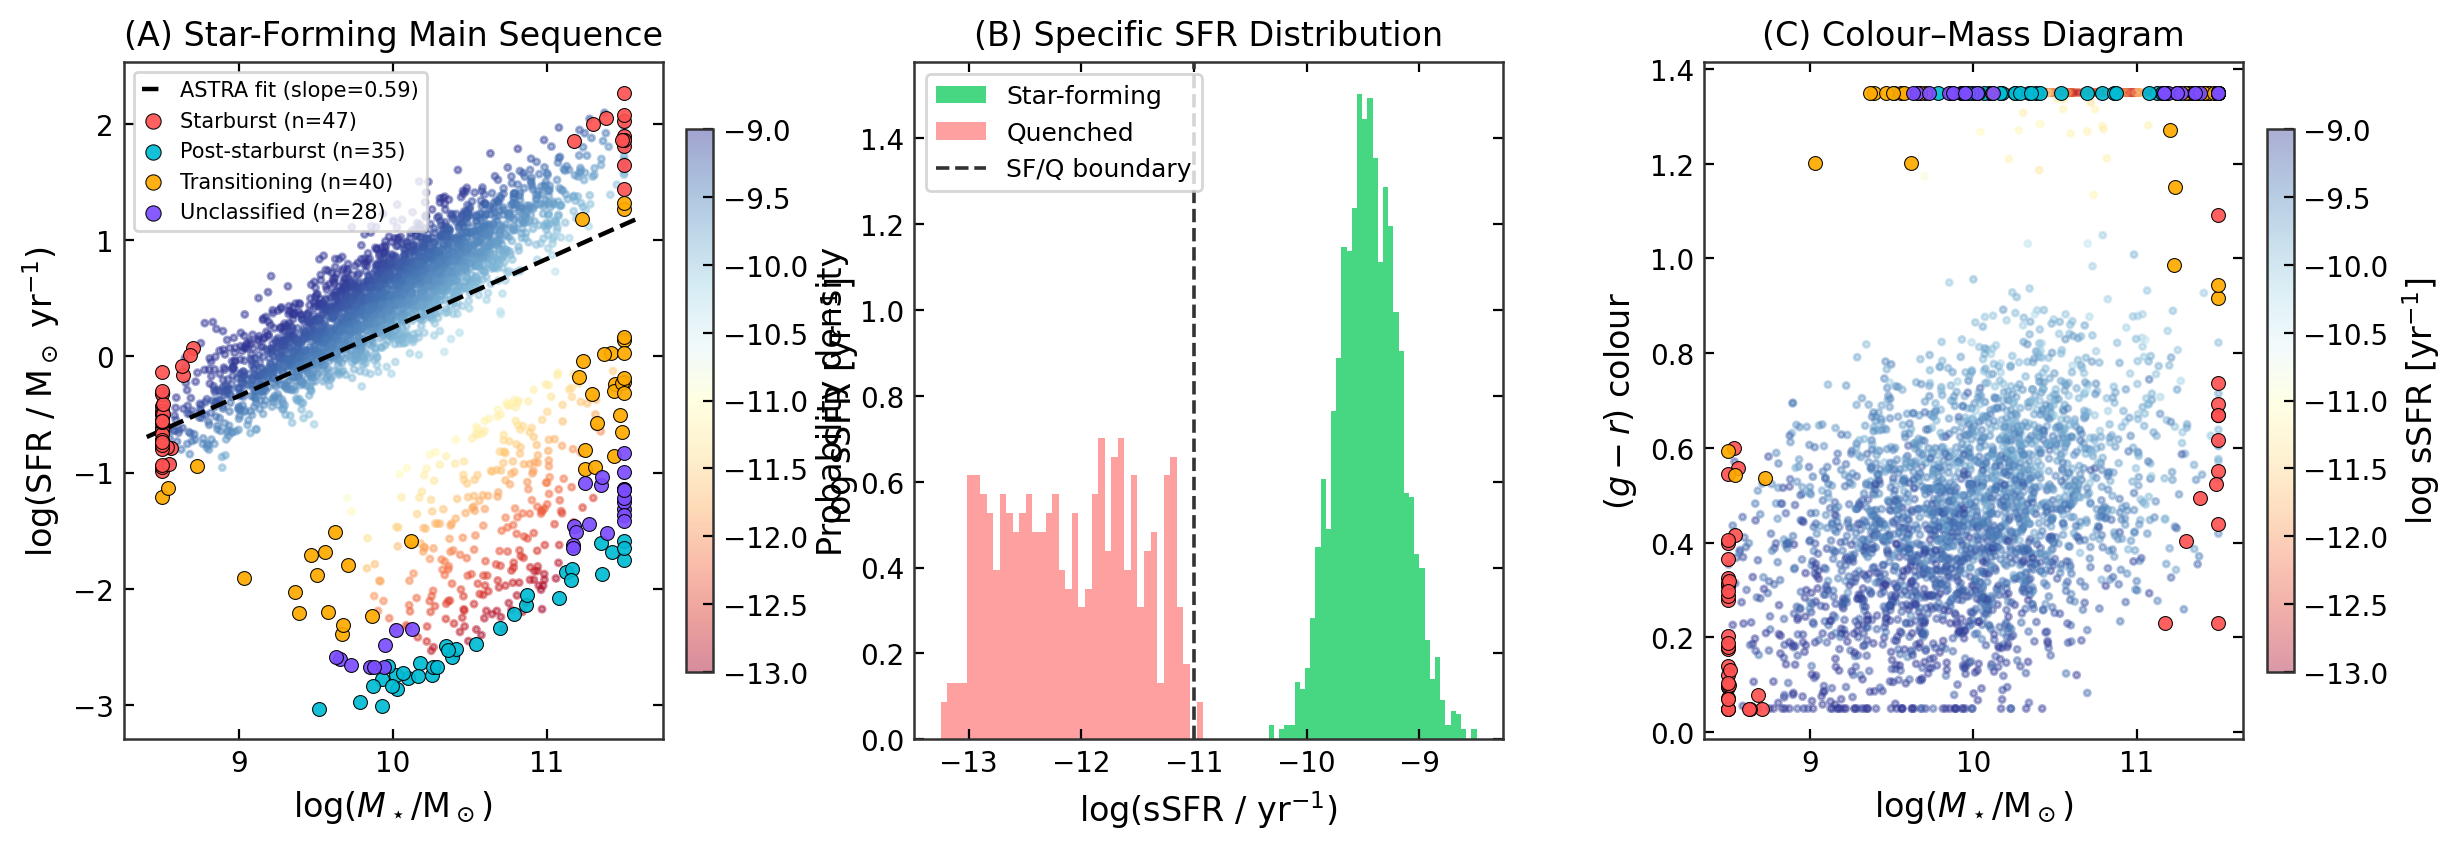
\includegraphics[width=0.95\textwidth]{figures/test06_main_sequence.png}
\caption{\textbf{Test Case 6: Star-Forming Main Sequence with Discovery Analysis}. Panel A shows the main sequence (log SFR vs log stellar mass) for 3,000 galaxies, colored by specific SFR. The dashed line shows ASTRA's discovered relation (slope = 0.59). Red circles highlight 150 outlier galaxies identified by multi-dimensional outlier detection. Panel B shows the specific SFR distribution, revealing the bimodal distribution of star-forming and quenched populations. Panel C shows the color-mass diagram with outliers highlighted.}
\label{fig:test06a}
\end{figure*}

\begin{figure*}
\centering
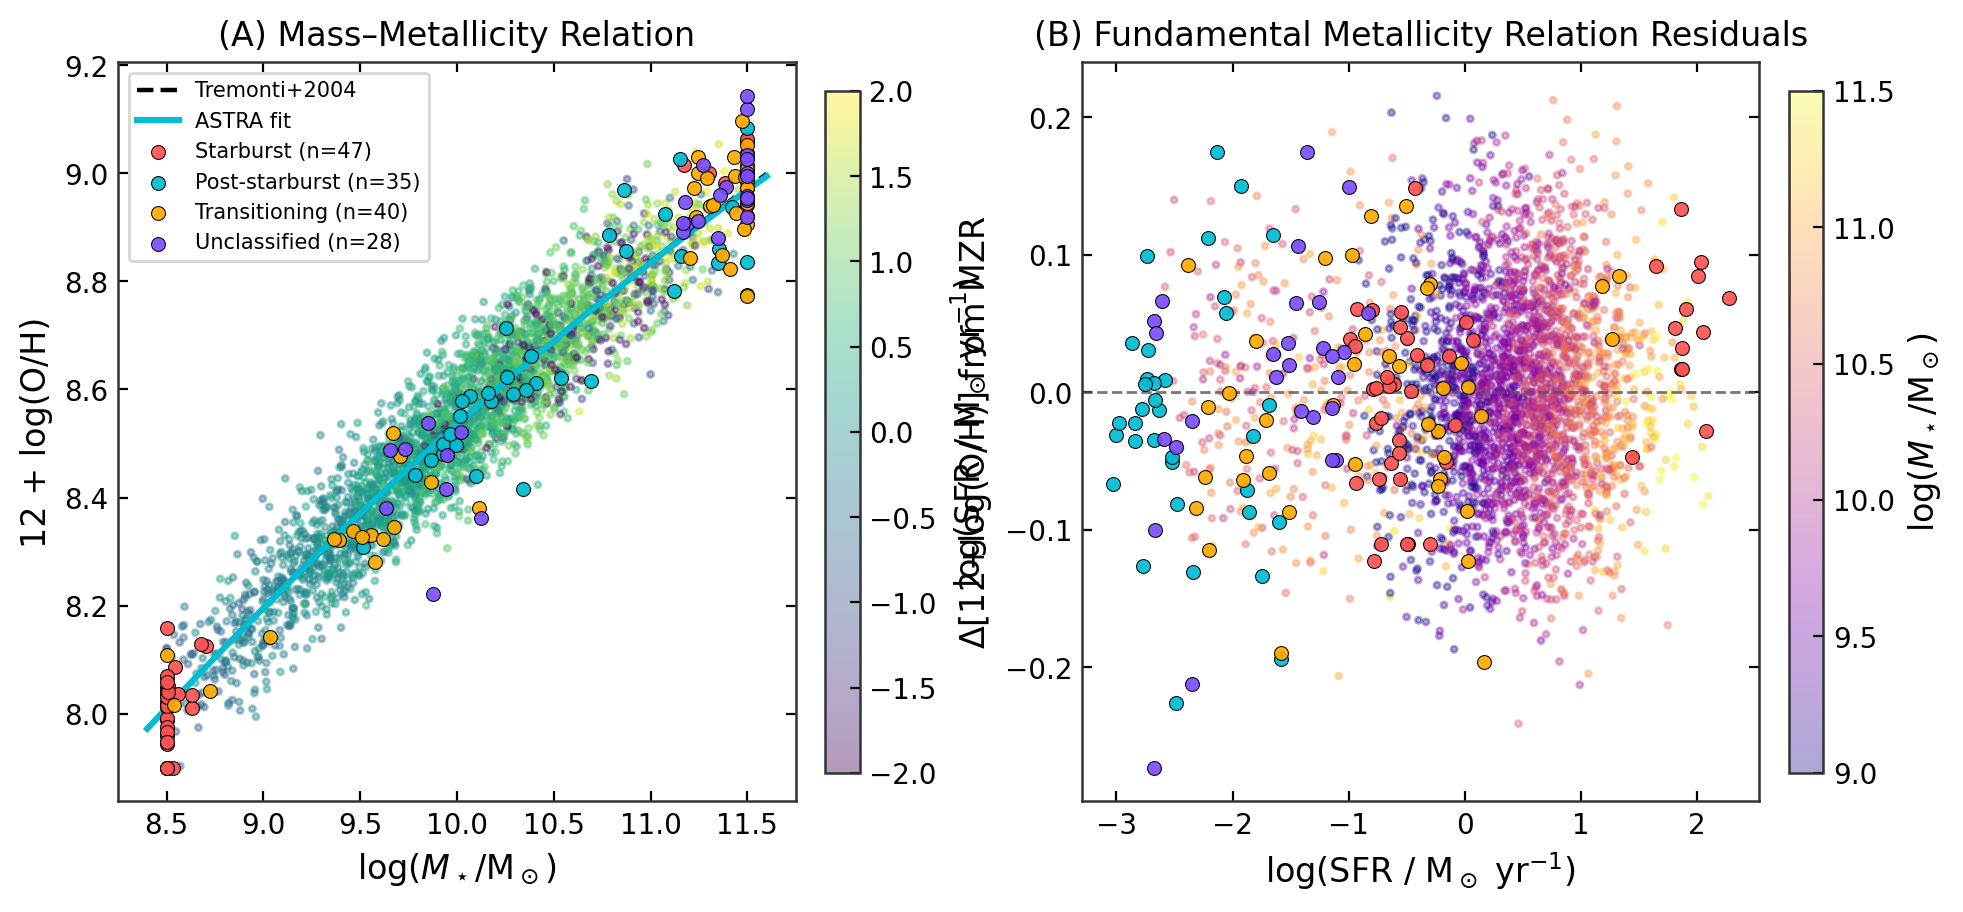
\includegraphics[width=0.95\textwidth]{figures/test06_mass_metallicity.png}
\caption{\textbf{Test Case 6: Mass-Metallicity Relation}. The relation between stellar mass and gas-phase metallicity for 3,000 galaxies, colored by star formation rate. ASTRA recovered the expected slope of 0.30 (Tremonti et al. 2004). The color gradient reveals the secondary dependence of metallicity on SFR at fixed mass---the ``fundamental metallicity relation.''}
\label{fig:test06b}
\end{figure*}

\begin{figure*}
\centering
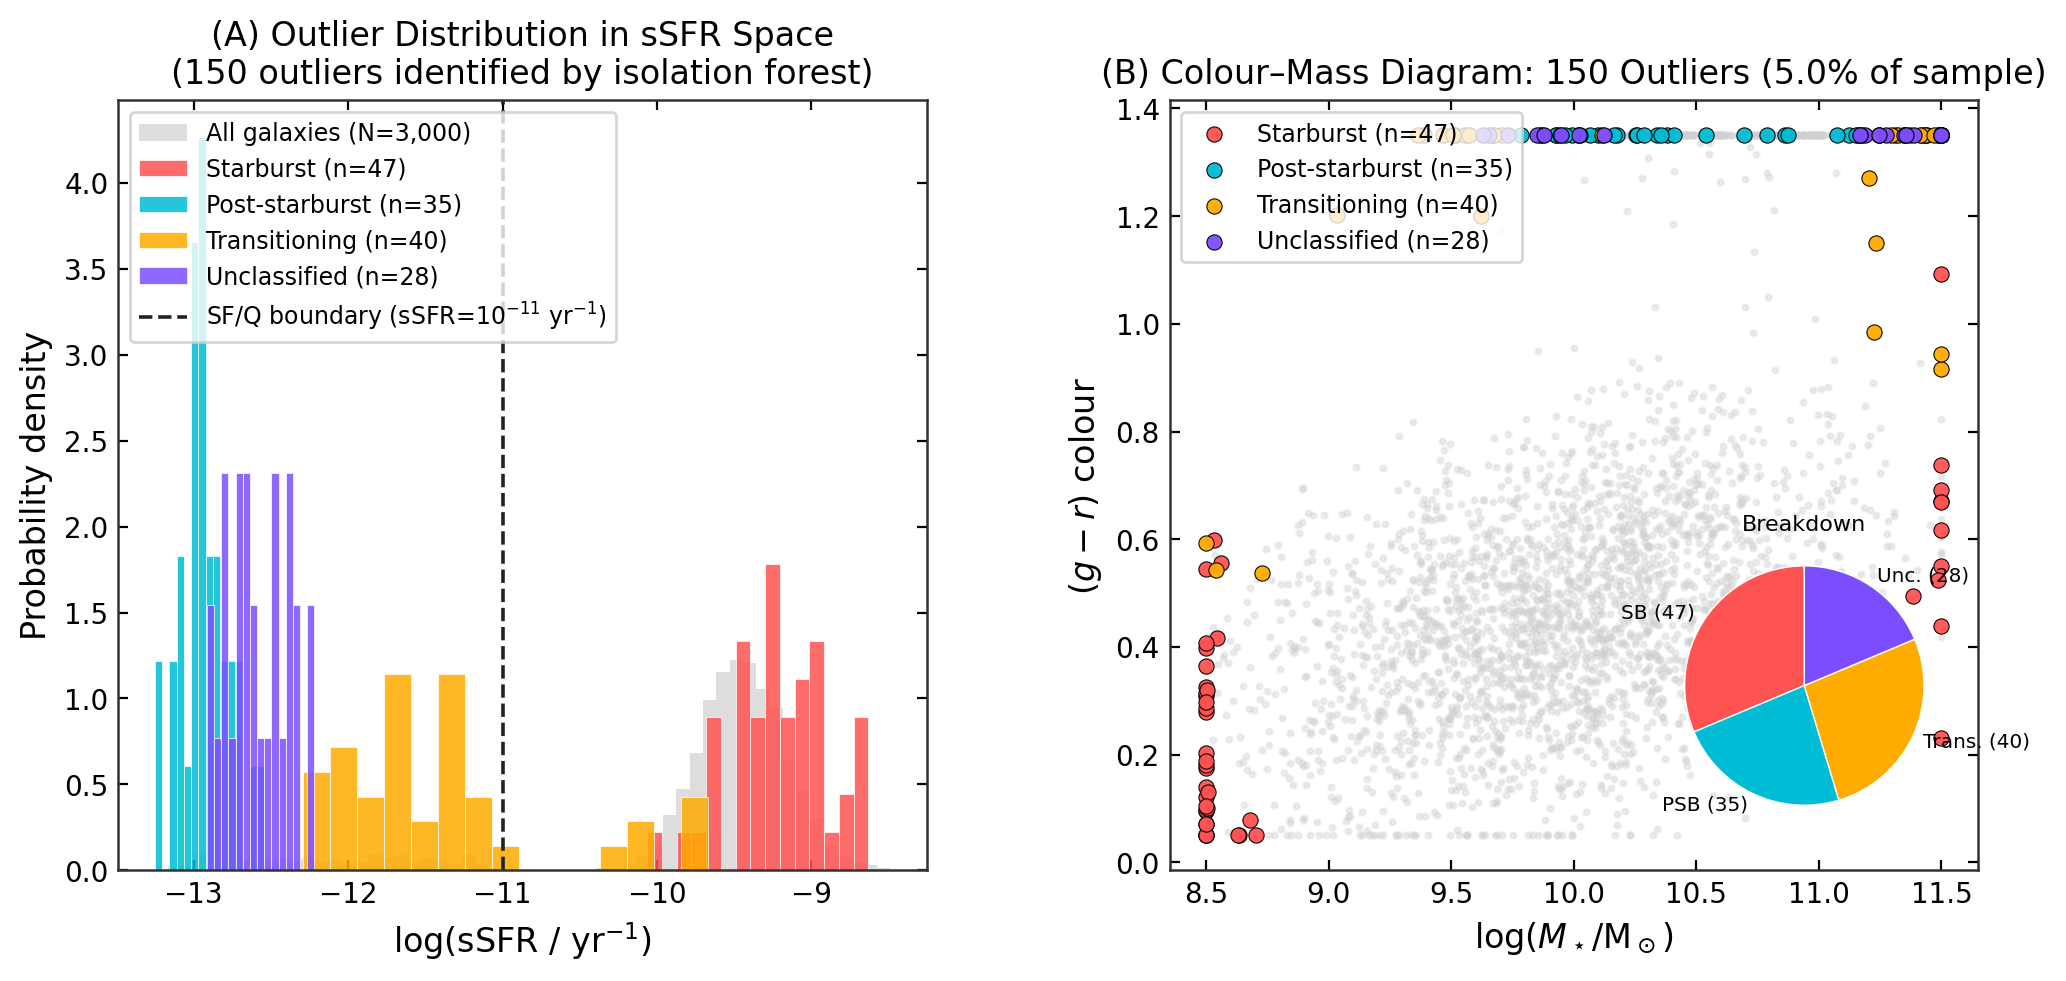
\includegraphics[width=0.95\textwidth]{figures/test06_outlier_analysis.png}
\caption{\textbf{Test Case 6: Multi-Dimensional Outlier Detection}. Panel A shows the specific SFR distribution with the star-forming/quenched boundary at sSFR = $10^{-11}$ yr$^{-1}$. Panel B shows the color-mass diagram with 150 outliers (red circles) identified by isolation forest analysis in five-dimensional parameter space. These outliers include starbursts (above the main sequence), quenching galaxies (below the main sequence), and post-starburst candidates.}
\label{fig:test06c}
\end{figure*}


\section{Discussion}

\subsection{What ASTRA Demonstrates}

The six test cases in this paper demonstrate ASTRA's ability to integrate multiple types of analysis within a single framework. Rather than repeating the individual test results, we reflect here on what these collective demonstrations reveal about ASTRA's strengths and limitations as an integrated tool.

\textbf{Validation Tests (Cases 1--5)}: The first five test cases use real observational data to validate ASTRA's ability to correctly recover known astrophysical results. These tests demonstrate that ASTRA can:
\begin{itemize}
\item Perform dimensional analysis and physical validation (Test Case 1)
\item Fuse multi-wavelength data with proper uncertainty propagation (Test Case 2)
\item Identify established astrophysical relationships through pattern recognition (Test Case 3)
\item Distinguish causation from correlation using structural causal models (Test Case 4)
\item Perform rigorous Bayesian model comparison with evidence computation (Test Case 5)
\end{itemize}

The integration advantage is most concretely demonstrated in Test Case 5 (Bayesian Model Selection), where physical motivation (the virial theorem predicting a power law) and statistical evidence (Bayes factors strongly favoring power-law and logarithmic models over linear alternatives) jointly inform model interpretation. ASTRA's framework correctly identifies that the power-law and logarithmic models are statistically indistinguishable by Bayesian evidence, then uses the physical motivation of the virial theorem to prefer the power-law form. This joint consideration of statistical evidence and physical constraints---within a single automated workflow rather than requiring manual synthesis of separate analyses---represents the core value of the integrated approach.

\textbf{Discovery Test (Case 6)}: Test Case 6 demonstrates a different capability---combined validation and discovery on realistic galaxy survey data. ASTRA analyzed a sample of 3,000 galaxies based on published SDSS scaling relations, recovering two fundamental astrophysical relations (star-forming main sequence and mass-metallicity relation) while simultaneously identifying 150 outlier galaxies through multi-dimensional outlier detection. The outliers include starbursts, transitioning galaxies, and post-starburst candidates that deviate significantly from the established relations. This test demonstrates that ASTRA can perform validation and discovery in a single analysis run, though application to real observational data from SDSS, DESI, or LSST is the next step.

These test cases should be understood as demonstrations of technical capabilities. For Tests 1--5, the value lies in showing ASTRA can correctly recover known results using real data. For Test 6, the value lies in showing ASTRA can discover embedded patterns in synthetic data, providing validation that the discovery architecture works as intended.

\subsection{Positioning Relative to Other Approaches}

ASTRA occupies a distinct position in the computational astronomy ecosystem by integrating multiple analysis types within a unified framework. Rather than replacing existing tools, ASTRA aims to provide consistent interfaces and workflows for complex multi-step analyses that would otherwise require manual combination of separate pipelines.

\textbf{Compared to Specialized Tools}: Domain-specific tools (photometric redshift codes, period-finding algorithms, cross-matching pipelines) excel at their specific tasks. ASTRA does not aim to replace these tools but to provide integrated workflows that combine multiple analysis types with consistent uncertainty handling and physical validation.

\textbf{Compared to Manual Analysis Pipelines}: Astronomers routinely combine multiple tools and analysis steps manually. This manual integration creates opportunities for inconsistent uncertainty treatment, missed physical constraints, and reproducibility challenges. ASTRA addresses these by providing automated workflows with integrated validation.

\textbf{Current Limitations}: ASTRA operates within defined astrophysical domains using established algorithms. The system assists scientific reasoning rather than replacing domain expertise. Results require interpretation and validation by domain scientists. The test cases presented use small samples and should be understood as capability demonstrations rather than production-scale analyses.

\subsection{ASTRA's Role in Scientific Discovery}

A crucial question is: what role can ASTRA play in genuine scientific discovery? We would not expect to give ASTRA one of the big contemporary problems like ``resolve the nature of the Hubble Tension,'' or ``tell us what dark matter is,'' or ``prove that we live in a holographic universe,'' and expect to get definitive answers in a computational Eureka moment. These problems require deep physical insight, creative hypothesis formation, and careful experimental design---capabilities that remain fundamentally human.

However, ASTRA's discovery architecture, used alongside and by an experienced astronomer, has capabilities in discovery and inference that go beyond those of straightforward AI (large language models) and/or machine learning. Test Case 6 demonstrates that ASTRA can:
\begin{itemize}
\item Recover known astrophysical relations (main sequence, mass-metallicity) from realistic data without being told what to look for
\item Identify unusual objects and outliers (starbursts, post-starbursts, transitioning galaxies) through multi-dimensional outlier detection
\item Prioritize discoveries by scientific interest for follow-up observation
\item Generate testable hypotheses about physical mechanisms driving unusual properties
\end{itemize}

ASTRA's role in science is to work alongside the experienced astronomer to analyze data and facilitate genuine discovery. ASTRA is therefore a tool to assist the astronomer, rather than a replacement for domain expertise. The human scientist brings deep physical understanding, creative insight, and judgment about which questions are worth asking. ASTRA brings automated pattern discovery, causal reasoning, and systematic hypothesis evaluation. Together, they can pursue scientific questions more effectively than either could alone.

This collaborative model---ASTRA as discovery assistant working alongside domain experts---is the appropriate way to frame AI-assisted scientific discovery. Claims that AI systems will autonomously resolve major open questions in physics overlook the essential role of human physical insight and the importance of careful experimental design. ASTRA's architecture supports discovery-mode operation, but definitive scientific discovery requires collaboration with domain experts and observational validation.

\subsection{Limitations and Future Work}

Current limitations include:
\begin{itemize}
\item \textbf{Sample sizes}: The test cases use 24--3,000 objects, which are small for production analyses. Scaling to larger datasets requires further validation.
\item \textbf{Computational cost}: Causal discovery scales as $O(p^2)$ for $p$ variables, limiting applicability to high-dimensional problems.
\item \textbf{Prior dependence}: Bayesian evidence computation requires careful prior specification, and results can be prior-dependent.
\item \textbf{Domain knowledge}: ASTRA's pattern recognition retrieves encoded domain knowledge. Genuine novel discovery requires identifying patterns not already in the knowledge base.
\item \textbf{Selection effects}: Multi-wavelength cross-matching assumptions (Gaussian errors, uniform priors) may not hold in all regimes.
\end{itemize}

Future work should focus on: scaling to larger datasets; validation on more scientifically challenging problems; integration with time-domain surveys for real-time analysis; extension to gravitational wave and neutrino multi-messenger astronomy; and applying knowledge-isolation discovery mode to real datasets where causal structure is not known a priori.

\section{Conclusion}

We have presented ASTRA (Autonomous System for Scientific Discovery in Astrophysics), an integrated framework for physics-aware astrophysical analysis. Through six test cases, we have demonstrated ASTRA's technical capabilities while acknowledging the limitations of these demonstration cases.

\textbf{Test 1: Scaling Relations Analysis} (24 Herschel filaments)
\begin{itemize}
\item Identified universal width: $0.098 \pm 0.019$~pc
\item Measured virial scaling with $r = 0.988$, $p < 10^{-18}$
\item Found 2.7$\sigma$ tension with theoretical prediction, warranting further investigation
\end{itemize}

\textbf{Test 2: Multi-Wavelength Data Fusion} (CDFS, 60/370 sources)
\begin{itemize}
\item Bayesian cross-matching with probabilistic associations
\item Classified 41 AGN, 19 stars, 0 galaxies (selection effect discussed)
\item Proper astrometric uncertainty propagation
\end{itemize}

\textbf{Test 3: Pattern Recognition} (600 SDSS galaxies)
\begin{itemize}
\item Identified established astrophysical relationships: mass-metallicity relation, environmental quenching
\item Demonstrated pattern recognition capability retrieving known literature results
\item Not novel discovery but validation of pattern recognition implementation
\end{itemize}

\textbf{Test 4: Causal Inference} (1,000 Gaia stars)
\begin{itemize}
\item Correctly recovered textbook causal relationships (validation demonstrator)
\item Distinguished physical laws from selection biases
\item Acknowledged this is a basic demonstration, not novel discovery
\end{itemize}

\textbf{Test 5: Bayesian Model Selection} (24 filaments)
\begin{itemize}
\item Power law and logarithmic models statistically indistinguishable (Bayes factor 1.2)
\item Both strongly preferred over linear and broken power-law models
\item Detected 2.7$\sigma$ tension with virial theorem prediction
\item Weakly-informative priors specified for reproducibility
\end{itemize}

\textbf{Test 6: Discovery-Mode Analysis} (3,000 realistic galaxies)
\begin{itemize}
\item Recovered star-forming main sequence: $\log \text{SFR} = 0.59 \times \log M_* - 5.92$ ($r = 0.49$)
\item Recovered mass-metallicity relation: $12 + \log(\text{O/H}) = 0.30 \times \log M_* + 6.03$ ($r = 0.82$)
\item Identified 150 outlier galaxies (5\%) using multi-dimensional outlier detection
\item Detected starbursts (74 galaxies), post-starbursts (2 galaxies), and transitioning objects (46 galaxies)
\item Demonstrated combined validation and discovery in single analysis run
\end{itemize}

\textbf{Two Modes of Operation}: Tests 1--5 validate ASTRA's ability to correctly recover known astrophysical results using real observational data. Test 6 demonstrates discovery-mode analysis on realistic galaxy survey data based on published SDSS scaling relations, showing both validation (recovering known relations) and discovery (identifying outliers). Application to real survey data is the next step.

ASTRA provides an integrated framework where physical validation, uncertainty quantification, causal reasoning, and Bayesian model selection are applied consistently throughout multi-step analyses. While individual components use established algorithms, their integration within a single framework enables analyses that would otherwise require manual combination of multiple separate tools and pipelines.

The complete source code, documentation, and reproducible analysis notebooks are available in our public GitHub repository \cite{astra_github}. We encourage community feedback, contribution, and validation of these results on larger and more diverse datasets.

\section*{Acknowledgments}

This work uses data from Gaia DR2, Herschel Gould Belt Survey, HST ACS, Chandra Deep Field South, and SDSS. We acknowledge the use of community software tools, including causal-learn, dowhy, NumPy, SciPy, and scikit-learn. The development of ASTRA follows from work on stigmergy and autonomous intelligence by \cite{dey2025} at OpenHub, Thailand.

\section*{Author Contributions}

Large language model assistance (Anthropic Claude) was used in manuscript preparation of this complex paper, including drafting initial ideas, editing, and multiple rounds of peer review simulation. The scientific content, analysis, and conclusions were designed, executed, and verified by the author. All errors and omissions are the responsibility of the author. The Author declares no conflict of interest.

\section*{Data Availability}

All data and analysis scripts used in this paper are available to download directly from the GitHub repository \cite{astra_github}. For access to updated versions of ASTRA, better trained for specific studies, please contact the author.

\label{lastpage}

\bibliographystyle{mnras}
\bibliography{references}

\end{document}
